
\documentclass[Portugues,Final]{tese-FT}
    % Para acrescentar comentários ao PDF descomente:
\usepackage
         [pdfauthor={Romulo Messias Silva Souza},
         colorlinks=false]
        %   pdftitle={titulo},
        %   pdfkeywords={palavra-chave, palavra-chave},
        %   pdfproducer={Latex with hyperref},
        %   pdfcreator={pdflatex}]
{hyperref}
        
        %Mantenha o pacote a seguir para citações no formato ABNT
\usepackage[alf]{abntex2cite}
        
        %Mantenha o pacote a seguir para incluir a lista de símbolos.
\usepackage{nomencl}
\makenomenclature
        
        %O pacote a seguir gera um dummy text. Elimine a linha quando
        % for editar seu texto.
\usepackage{lipsum}
\usepackage{algorithmicx}
\usepackage[Algorithm,ruled]{algorithm}
\usepackage{algpseudocode}
\usepackage{indentfirst}
\usepackage{multirow}
\usepackage{float}
\usepackage{longtable} 
\usepackage{tabto}

% Declaracoes em Português
\algrenewcommand\algorithmicend{\textbf{fim}}
\algrenewcommand\algorithmicdo{\textbf{faça}}
\algrenewcommand\algorithmicwhile{\textbf{enquanto}}
\algrenewcommand\algorithmicfor{\textbf{repita}}
\algrenewcommand\algorithmicif{\textbf{se}}
\algrenewcommand\algorithmicthen{\textbf{então}}
\algrenewcommand\algorithmicelse{\textbf{senão}}
\algrenewcommand\algorithmicreturn{\textbf{devolve}}
\algrenewcommand\algorithmicfunction{\textbf{função}}
% \algrenewcommand\algorithmc{Pseudocódigo}
% Rearranja os finais de cada estrutura
\algrenewtext{EndWhile}{\algorithmicend\ \algorithmicwhile}
\algrenewtext{EndFor}{\algorithmicend\ \algorithmicfor}
\algrenewtext{EndIf}{\algorithmicend\ \algorithmicif}
\algrenewtext{EndFunction}{\algorithmicend\ \algorithmicfunction}

% O comando For, a seguir, retorna 'para #1 -- #2 até #3 faça'
\algnewcommand\algorithmicto{\textbf{até}}
\algrenewtext{For}[3]%
{\algorithmicfor\ #1  }

\begin{document}
        
        % Escolha entre autor ou autora:
\autor{Romulo Messias Silva Souza}
        %\autora{Nome da Autora}
        % Sempre deve haver um título em português:
\titulo{DESENVOLVIMENTO DE OPERADORES DE BUSCA PARA DEFINIcaO DE ESTRATeGIAS DE PRODUO VIA ALGORITMOS GENTICOS}
        
        % Se a língua for o inglês ou o espanhol defina:
        %\title{The Dissertation or Thesis Title in English or Spanish for FT}
        
        % Escolha entre orientador ou orientadora e inclua os títulos:
\orientador{Prof. Dr. Guilherme Palermo Coelho}
        %\orientadora{Profa. Dra. Nome da Orientadora}
        
        % Escolha entre coorientador ou coorientadora, se houver, 
        % e inclua os títulos:
        %\coorientador{Prof. Dr. Eng. Lic. Nome do Co-Orientador}
        %\coorientadora{Prof. Dra. Eng. Lic. Nome da Co-Orientadora}
        
        % Escolha entre uma das quatro opções a seguir (comente as demais):
        %\bsi         % para Trabalho de Conclusão de Curso em BSI
        %\tads       % para Trabalho de Conclusão de Curso em TADS
        %\qualificacaoMestrado  % Para textos de qualificação de mestrado.
        %\qualificacaoDoutorado % Para textos de qualificação de doutorado.
        \mestrado   % para Dissertação de Mestrado em Tecnologia
        %\doutorado  % para Tese de Doutorado em Tecnologia
        
        % Se houve cotutela, defina:
        %\cotutela{Universidade Nova de Plutão}
        
        %Defina a data da defesa no formato {Dia}{Mês}{Ano}
        \datadadefesa{00}{06}{2018}
        
        % Para a versão final defina:
        % Repita o nome do Orientador(a) no primeiro avaliador
        \avaliadorA{Prof. Dr. Nome do Orientador}{FT/UNICAMP}
        \avaliadorB{Profa. Dra. Segunda Avaliadora}{Instituição da segunda avaliadora}
        \avaliadorC{Dr. Terceiro Avaliador}{Instituição do terceiro avaliador}
        %\avaliadorD{Prof. Dr. Quarto Avaliador}{Instituição do quarto avaliador}
        %\avaliadorE{Prof. Dr. Quinto Avaliador}{Instituição do quinto avaliador}
        %\avaliadorF{Prof. Dr. Sexto Avaliador}{Instituição do sexto avaliador}
        %\avaliadorG{Prof. Dr. Sétimo Avaliador}{Instituição do sétimo avaliador}
        %\avaliadorH{Prof. Dr. Oitavo Avaliador}{Instituição do oitavo avaliador}
        
        
        % Para incluir a ficha catalográfica em PDF na versão final, 
        % copie o arquivo PDF, descomente e ajuste a linha a seguir:
        %\fichacatalografica{arquivo.pdf}
        
        % Este comando deve ficar aqui:
        \paginasiniciais
        
        % Se houver dedicatória, descomente a linha a seguir:
        %\prefacesection{Isso é um teste}
        %A dedicatória deve ocupar uma única página.
        %
        %
        % Se houver epígrafe, descomente e edite as linhas a seguir:
         \begin{epigrafe}
        {\it
        Vita brevis,\\
        ars longa,\\
        occasio praeceps,\\
        experimentum periculosum,\\
        iudicium difficile.}
        
        \hfill (Hippocrates)
        \end{epigrafe}
        %
        %
        % Agradecimentos ou Acknowledgements ou Agradecimientos
        \prefacesection{Agradecimentos}
        Os agradecimentos devem ocupar uma única página.
        
        % Sempre deve haver um resumo em português:
        \begin{resumo}
        O planejamento da estratégia de extração de petróleo em campos de águas profundas é uma das etapas essenciais da engenharia de reservatórios. É nessa etapa que são definidos os parâmetros de construção e operação do sistema de produção que será implantado no campo, de forma a otimizar algum critério, como o lucro gerado pelo campo ou o volume total de óleo que será extraído durante o período de concessão. Apesar de ser possível utilizar ferramentas clássicas para resolver esse problema de otimização, para que tais métodos funcionem diversas simplificações devem ser consideradas, principalmente, por conta dos níveis de incerteza relacionados ao problema. Tais simplificações pode levar a soluções que não condizem com a realidade.Meta-heurísticas são ferramentas alternativas de otimização que se mostram adequadas para problemas onde os métodos clássicos não são se mostram eficientes, uma vez que, ao contrário das metodologias clássicas de otimização, as meta-heurísticas não exigem grandes adaptações para serem aplicadas ao problema que se deseja resolver. no entanto, é comum que tais ferramentas exijam um elevado número de avaliações de soluções candidatas até que uma solução adequada seja obtida. Esta característica é particularmente desfavorável para o problema de definição de estratégia de produção, uma vez que a avaliação de uma solução exige a simulação computacional da evolução do campo de petróleo durante todo o período de exploração. Essa simulação pode levar várias horas dependendo do nível de detalhamento do modelo do campo. Sendo assim, esse trabalho propõe a estudar o uso de meta-heurísticas para a resolução do problema de definição de estratégia de produção com o objetivo de reduzir o custo computacional para que uma solução de boa qualidade seja encontrada. De forma mais específica, aqui foi desenvolvido versões específicas do algoritmo genético, bem como de seus operadores de busca, para o problema em questão. Tais modificações utilizam de conhecimento acerca do problema para explorar de forma mais eficiente o espaço de busca. As versões clássica do algoritmo genético e as modificações propostas foram utilizadas para otimizar uma estratégia de produção em um modelo sintético de reservatório de petróleo, os resultados foram então apresentados e comparados com uma busca aleatória e uma ferramenta comercial de otimização.
        \\ \\ 
        \textit{Palavras Chave:} Otimização, Meta-heurísticas, Engenharia de Reservatórios, Estratégia de Produção
        \end{resumo}
        
        
        % Sempre deve haver um abstract:
        \begin{abstract}
        Planning the oil extraction strategy to be deployed in deep-water fields is one of the most important steps of reservoir engineering. In this step, several parameters related to the construction and operation of the production system to be implemented must be defined. These parameters are adjusted to optimize some criteria, such as profit by the field or the total volume of oil that will be extracted during the concession period. Although it is possible to use classic tools to solve this optimization problem, these methods need several simplifications to work properly, mainly, due to all the uncertainties associated with this problem. Such simplifications can lead to solutions that do not satisfy reality. Meta-heuristics are alternative optimization tools suitable for problems where classic tools are not efficient. Because meta-heuristics, in contrast to classic tools, require little adaptation to be applied to a particular problem. However, such algorithms often require a high number of objective function evaluations to obtain high-quality solutions. This characteristic is particularly adverse for production strategy definition problem, since the evaluation of each candidate solution requires a computational simulation of the evolution of the oil field throughout the period of operation. Each simulation can take several hours to complete, according to the level of details adopted for the field’s model. Therefore, this project aims to reduce computational cost in the search processo to find good solutions for production strategy definition problem by using meta-heuristics. In a more specific way specific versions of the genetic algorithm was developed for this problem. This modified version of the algorithms uses problem knowledge to explore the search space more efficiently. Both the classical versions of the genetic algorithm and the versions proposed here were used to optimize a production strategy in a synthetic model of oil reservoir. The results were then presented and compared with a random search and commercial optimization tool.
        \\ \\
        \ textit {Keywords:} Optimization, Metaheuristics, Reservoir Engineering, Production Strategy
        \end{abstract}
        
        % Se houver um resumo em espanhol, descomente as linhas a seguir:
        %\begin{resumen}
        % A mesma regra aplica-se.
        %\end{resumen}
        
        % A lista de figuras:
        \listoffigures
        
        % A lista de tabelas:
        \listoftables
        
        % A lista de abreviações e siglas é opcional:
        
        % $ABC$	COlônia de Abelhas Artificiaiadadasaas
        \prefacesection{Lista de Abreviações e Siglas}
\NumTabs{5}
$ABC$ \tab{Colônia de Abelhas Artificiais} \bigbreak
$ACO$  \tab{ Otimização por Colônia de Formigas \bigbreak
$AG$  \tab{ Algoritmos Genéticos} \bigbreak
$AG^{RPC}$  \tab{ Algortimo Genético de Regime Permanente Clássico} \bigbreak
$AG^{RPC-x}$  \tab{ $AG^{RPC}$ executado com as configuraç~eos do experimento $x$} \bigbreak
$AG^{GC}$  \tab{ Algoritmo Genético Geracional Clássico \bigbreak
$AG^{GC-x}$  \tab{ $AG^{GC}$ executado com as configurações do experimento $x$} \bigbreak
$AG^{RPM}$  \tab{ Algoritmo Genético de Regime Permanente Modificdo} \bigbreak
$AG^{RPM730}$  \tab{ $AG^{RPM}$ executado com o máximo de 730 avaliações da função objetivo} \bigbreak
$AG^{CO}$  \tab{ $AG^{RPM}$ com Contador de Ocorrências} \bigbreak
$AG^{CO-t}$  \tab{ $AG^{CO}$ com o tamanho de população t} \bigbreak
$AG^{BL}$  \tab{ $AG^{RPM}$ com Busca Local} \bigbreak
$AG^{BL-v}$  \tab{ $AG^{BL}$ com a versão v da busca local} \bigbreak
$BA$  \tab{ Busca Aleatória} \bigbreak
$CMG$  \tab{ \textit{Computer Modelling Group}} \bigbreak
$CMOST$  \tab{ Software de ajuste de histórico e otimização da $CMG$} \bigbreak
$CMOST^{500}$  \tab{ $CMOST$ executado com o máximo de 500 avaliações da função objetivo} \bigbreak
$CMOST^{730}$  \tab{ $CMOST$ executado com o máximo de 730 avaliações da função objetivo} \bigbreak
$CO$  \tab{ Custos Assoiados a Produção} \bigbreak
$COFINS$  \tab{ Contribuição para Financiamento da Seguridade Social Exploração} \bigbreak
$DEP$  \tab{ Definição de Estratégia de Prodção} \bigbreak
$DEPeq$  \tab{ Depreciação de Equipamentos} \bigbreak
$EE$  \tab{ Estratégias Evolutivas} \bigbreak
$EPP$  \tab{ Indicador de Performance do Poço} \bigbreak
$FCt$  \tab{ Fluxo de Caixa no instante de tempo t} \bigbreak
$GRASP$  \tab{ greedy randomized adaptive search procedures} \bigbreak
$IC$  \tab{ Investimentos Contabilizados} \bigbreak
$ICA$  \tab{ IMperialist Competitive Algorithm} \bigbreak
$ICMS$  \tab{ Imposto de Renda e Contribuição Social} \bigbreak
$ID$  \tab{ Investimentos Depreciáveis} \bigbreak
$IEP$  \tab{ Indicador Ecônomico dos Poços} \bigbreak
$IEPI$  \tab{ Indicador Ecônomico dos Poços Injetores} \bigbreak
$IEPP$  \tab{ Indicador Ecônomico dos Poços Produtores} \bigbreak
$IMEX$  \tab{ Simulador comercial Black-Oilda desenvoldido pela $CMG$} \bigbreak
$MADS$  \tab{ Mesh Adaptative Direct} \bigbreak
$MERO$  \tab{ Ferramenta desenvolvida pelo Grupo UNISIM} \bigbreak
$PASEP$  \tab{ Programa de Formação do Patrimônio do Servidor Público} \bigbreak
$PE$  \tab{ Programação Evolutiva} \bigbreak
$PES$  \tab{ Participação Especial} \bigbreak
$PIS$  \tab{ Programa de Ingregração Social} \bigbreak
$PPC$  \tab{ PIS/PASEP e COFINS} \bigbreak
$PSO$  \tab{ Otimização por Enxame de Partículas} \bigbreak
$r$  \tab{ Taxa de desconto} \bigbreak
$R$  \tab{ Receita} \bigbreak
$RNA$  \tab{ Redes Neurais Artificiais} \bigbreak
$SA$  \tab{ Simulated Annealing} \bigbreak
$VPL$  \tab{ Valor Presente Líquido} \bigbreak
$VPLPP$  \tab{ VPL do poço Produtor} \bigbreak

        % A lista de símbolos é opcional:
        % \prefacesection{Lista de Símbolos}
        
        % Quem usa o pacote nomencl para abreviaturas pode incluir:
        % \renewcommand{\nomname}{Lista de Abreviações e Siglas}
        % \printnomenclature[3cm]
        
        % O sumário vem aqui:
        \tableofcontents
        
        % E esta linha deve ficar bem aqui:
        \fimdaspaginasiniciais
        
        % O corpo da dissertação ou tese começa aqui:
        %
        % O comando a seguir inclui o arquivo introducao.tex
        % que contém o capítulo de Introdução. 
        % Detalhe: não precisa incluir a extensão .tex
        
\chapter{Introdução}
\label{ch:ch1}
O petróleo é uma das principais fontes de combustível, representando cerca de um terço do total do consumo de combustível mundial. Em 2016, o consumo global desse combustível aumentou 1,6\% em relação a 2015, totalizando em 96,6 milhões de barris de petróleo por dia~\cite{BritishPetroleum2017, ANP2017}. No entanto, para o mesmo período, a produção global de petróleo não cresceu na mesma velocidade. Em 2016 foram produzidos 92,2 milhões de barris de petróleo por dia e, apesar de um aumento de 0,4\% em relação a 2015, a produção foi aquém da demanda.

Em virtude disso é importante buscar por formas de otimizar a produção de petróleo para suprir toda a demanda do mercado. A produção desse combustível não é uma tarefa fácil. Desenvolver e gerenciar campos de petróleo é uma atividade de risco, exige altos investimentos e traz uma série de desafios. Para que o produto chegue até o mercado há uma série de etapas que vão desde a descoberta e aquisição de dados sobre o reservatório de petróleo, a definição de uma estratégia de produção para a exploração do campo e o processamento e refinamento do óleo\cite{ANP2017}.

Dentre essas etapas, definir a estratégia de produção é um passo importante para explorar de forma eficiente o campo de petróleo. Uma vez definida, espera-se que tal estratégia seja utilizada por todo o período de exploração do campo. De forma sucinta, a definição da uma estratégia de produção (DEP) pode ser modelada como um problema de otimização, cujo objetivo final é definir e dimensionar o sistema de produção a ser adotado em um campo de petróleo de forma a maximizar algum critério. Tal critério, na maioria das vezes, é o Valor Presente Líquido (VPL), que é, essencialmente, o lucro obtido ao final da exploração do campo \cite{Marques2012}.

Dimensionar o sistema de produção para a exploração do campo também não é uma tarefa simples devido ao grande número de variáveis, relacionadas às características do sistema de produção, e às incertezas associadas ao problema e que dizem respeito às propriedades físicas do reservatório, à dinâmica do mercado e aos eventuais problemas com os equipamentos. Além disso, o próprio modelo que descreve o campo contém incertezas significativas, dado que é uma tentativa de representar algo que se encontra a quilômetros de profundidade.

Apesar de ser possível utilizar ferramentas clássicas para resolver esse problema de otimização, como Programação Inteira Mista \cite{Rosenwald1974} ou métodos baseados em gradiente \cite{Bangerth2006, Handels2007}, para que tais métodos funcionem diversas simplificações devem ser consideradas, o que pode levar a soluções que não condizem com a realidade ou, ainda, corre-se o risco do algoritmo ficar preso em uma solução de ótimo local \cite{Nasrabadi2012}. Dito isso, é necessário recorrer a ferramentas alternativas para obtenção de boas soluções para o problema de DEP como, por exemplo, as meta-heurísticas \cite{Blum2003}. Meta-heurísticas são ferramentas de propósito geral, ou seja, ferramentas que podem ser aplicadas a diferentes problemas sem a necessidade de grandes adaptações, independentemente das características intrínsecas do problema em questão (convexidade, diferenciabilidade, multimodalidade etc.). Dentre as meta-heurísticas, cabe destacar as meta-heurísticas populacionais, como os algoritmos genéticos, que atuam em cima de uma população de soluções candidatas para o problema, refinando-as sucessivamente até que uma solução suficientemente boa seja encontrada \cite{Back2000, decastro2006-CRC-fundamentals}. Além disso, variantes de tais ferramentas buscam manter diversidade entre as soluções candidatas na população, o que as tornam menos suscetíveis aos ótimos locais do problema e capazes de retornar, em uma única execução, múltiplas soluções distintas e de boa qualidade \cite{DeFranca2010}.

Muitas dessas características fazem com que as meta-heurísticas tenham grande potencial de aplicação ao problema de DEP, principalmente quando combinadas aos resultados gerados por simuladores de campos de petróleo e por outras ferramentas auxiliares que retornam, por exemplo, o VPL associado a uma dada estratégia de produção. Nesse contexto, as meta-heurísticas são responsáveis por buscar estratégias de produção, ou seja, definir os parâmetros do sistema de produção, enquanto que os módulos auxiliares são responsáveis por avaliar tais estratégias.

Por outro lado, o fato de serem ferramentas de propósito geral faz com que as meta-heurísticas tendam a demandar um número relativamente alto de avaliações de soluções candidatas até que uma solução de boa qualidade seja encontrada e retornada. Não é incomum encontrar, na literatura, aplicações de meta-heurísticas que envolvam dezenas de milhares de avaliações de soluções candidatas durante o processo de otimização \cite{Coelho2010}. A exigência de um alto número de avaliações de função é crítica para a aplicação de meta-heurísticas a problemas de DEP. Em tais situações, cada avaliação de uma solução candidata exige uma execução do software de simulação do campo de petróleo, que pode levar de alguns minutos a várias horas dependendo do nível de detalhamento do modelo do campo em estudo. 

Sendo assim, esse trabalho tem como objetivo estudar formas de aplicação de meta-heurísticas ao problema de definição de estratégias de produção (DEP) em campos de petróleo com o intuito de diminuir o custo computacional necessário para que o algoritmo encontre uma solução de boa qualidade. Para tal, dentre as meta-heurísticas disponíveis na literatura, foram escolhidos os algoritmos genéticos para serem aplicados ao problema de DEP. Aqui são propostos operadores de busca específicos para o problema de DEP e uma versão modificada de algoritmo genético. Para que tais objetivos pudessem ser atingidos foram realizados estudos sobre as principais meta-heurísticas disponíveis na literatura para tratar problemas de otimização e sobre gerenciamento de campos de petróleo, para identificar características do problema de DEP que podem auxiliar no processo de otimização. O algoritmo genético e os operadores propostos foram utilizados para otimizar o posicionamento de poços de uma estratégia de produção em um reservatório de petróleo sintético, sendo que tanto o escopo do problema quanto o modelo utilizado foram definidos em conjunto com os engenheiros do grupo UNISIM\footnote{UNISIM é um grupo de pesquisa em simulações numéricas para reservatórios de petróleo. O grupo pertence ao Departamento de Energia, Divisão de Engenharia de Petróleo, da Faculdade de Engenharia Mecânica da UNICAMP e ao Centro de Estudos de Petróleo. Mais informações em: www.unisim.cepetro.unicamp.br/br/}.

Este documento está estruturado da seguinte forma: o Capítulo \ref{ch:ch1}, que se seguiu, contextualizou o trabalho e apresentou suas motivações e objetivos; os conceitos teóricos e a revisão bibliográfica sobre Meta-heurísticas e Gerenciamento de Campos de Petróleo são discutidos no Capítulo 2; os operadores desenvolvidos aqui, bem como as modificações realizadas ao Algoritmo Genético são apresentados no Capítulo 3; no Capítulo 4 são descritas as ferramentas computacionais utilizadas para o desenvolvimento desse trabalho, bem como o caso de estudo e a estrutura dos experimentos realizados; os resultados obtidos são discutidos no Capítulo 5; e, por fim, as conclusões são comentadas no Capítulo 6.
        \chapter{Revisão Bibliográfica}
\label{ch:ch2}
Nesse capítulo são apresentadas as principais características das meta-heurísticas, com um foco maior no algoritmo escolhido para aplicação ao problema de DEP: os Algoritmos Genéticos. Além disso são discutidas também as características e dificuldades do gerenciamento de campos de petróleo, bem com uma revisão dos principais trabalhos que se propuseram a resolver o problema de DEP com o uso de meta-heurísticas.

\section{Meta-heurísticas}
\label{sec:section21}
Diariamente lidamos com uma série de problemas dos mais diversos tipos. Para \cite{Michalewicz2004}, um problema existe quando há uma diferença entre um estado atual e um estado no qual se deseja estar. Ainda segundo \cite{Michalewicz2004}, alocar recursos que estejam disponíveis para diminuir a diferença entre esses estados é o que chamamos de solução. É comum que exista mais de uma solução viável para a resolução de um problema, nesse caso, é sempre desejável que a solução ótima, ou a mais próxima disso, seja a escolhida para ser executada.

Nesse cenário, em que há diversas soluções candidatas para resolver um determinado problema, encontrar a solução ótima é um problema por si só. Esse problema em questão é conhecido como problema de otimização.  Tal otimização consiste em buscar pela solução ótima dentro de um conjunto de soluções (que formam o chamado espaço de busca), visando atender a algum critério. Geralmente tal critério é um determinado aspecto de interesse (objetivo) como lucro, desempenho, tempo ou distância, que deve ser maximizado ou minimizado. Na maioria das vezes é possível representar esse objetivo através de uma função matemática, conhecida como função objetivo e responsável por atribuir um número real a cada solução candidata do problema, indicando, dessa forma, o quão bem uma determinada solução resolve o problema.

São diversos os métodos que existem para resolver problemas de otimização. É possível partir para estratégias mais simples como a realização de uma busca por força bruta, enumerando e avaliando todas as soluções candidatas e escolhendo a melhor entre as opções, ou mesmo utilizar métodos mais clássicos como os baseados em gradiente. No entanto, a utilização de métodos como esses pode se mostrar ineficiente e até mesmo infactível, dependendo do problema que se deseja otimizar. \cite{Michalewicz2004} relatam algumas das características que tornam certos problemas de otimização difíceis de serem resolvidos:

\begin{itemize}
\item O problema possui uma quantidade grande de soluções candidatas;
\item O problema precisa ser simplificado para que se obtenha um conjunto de soluções candidatas. No entanto, as soluções geradas podem não ser boas o suficiente para solucionar o problema.
\item O problema possui restrições que exigem a realização de operações especiais para gerar soluções factíveis.
\end{itemize}

Problemas com essas características tornam inviável a avaliação de todas as soluções candidatas ou não permitem a definição de uma função objetivo que seja diferenciável, característica essencial para métodos baseados em gradiente, uma vez que esses métodos utilizam a derivada da função objetivo para direcionar a busca pela solução ótima. Para esse tipo de problema, é possível utilizar um grupo de métodos conhecidos por meta-heurísticas. 

Definir o que são meta-heurísticas não é uma tarefa simples. O termo foi vagamente introduzido por \cite{Glover1986} ao descrever a Busca Tabu como uma sobreposição de outra heurística. \cite{sorensen2013metaheuristics} propuseram uma definição mais concreta para o termo:


“Uma meta-heurística é uma estrutura algorítmica de alto nível e independente do problema que fornece um conjunto de orientações e estratégias para desenvolver algoritmos de otimização heurística. O termo também é utilizado para referir-se à implementação para um problema específico de tais algoritmos segundo as orientações destes” \cite{sorensen2013metaheuristics}.

De forma geral, é possível dizer que meta-heurísticas são metodologias de alto nível que podem ser usadas para desenvolver heurísticas a fim de resolver um problema específico de otimização \cite{Talbi2009}. Tais metodologias fazem parte de um campo maior de estudo conhecido por Otimização Estocástica \cite{Luke2013Metaheuristics}. A principal característica de algoritmos de otimização estocástica é o uso de técnicas que utilizam probabilidades para realizar operações durante o processo de busca por soluções ótimas. O uso de tal metodologia é comum em problemas de otimização para os quais nenhum outro método clássico pode ser aplicado com sucesso.

As meta-heurísticas tradicionalmente conseguem ser aplicadas a estes problemas por serem ferramentas de propósito geral que não exigem grandes adaptações, diferentemente de grande parte dos métodos clássicos de otimização. Ademais, as meta-heurísticas possuem estratégias que procuram escapar de soluções que representem ótimos locais do espaço de busca. Em contrapartida, principalmente pelo caráter estocástico destas metodologias, não há garantias de que a solução ótima, ou mesmo uma solução aceitável, será encontrada durante o processo de busca \cite{Talbi2009}. 

Apesar de não exigirem grandes adaptações, outros desafios surgem ao lidar com meta-heurísticas. Dentre eles, há a escolha de uma representação da solução candidata do problema, a definição da função objetivo a ser otimizada, as formas como as restrições do problema serão tratadas e a definição de parâmetros do algoritmo. Estes quatro pontos são detalhados a seguir.

\subsection{Representação da solução candidata}
\label{subsec:subc211}
A forma como uma solução candidata para o problema será representada computacionalmente ditará grande parte da estratégia de busca da meta-heurística, definindo diretamente o tamanho do espaço de busca que deve ser explorado e os operadores de busca que deverão ser utilizados. Uma solução candidata pode ser codificada de várias formas, sendo que grande parte dos problemas podem ter soluções representadas por codificações clássicas presentes na literatura, tais como cadeias binárias, vetores de valores discretos, vetores de valores reais ou permutações de valores inteiros. \cite{Talbi2009} sugere que uma representação da solução candidata deve possuir as seguintes características:

\begin{itemize}
\item \textbf{Plenitude:} relacionada à capacidade de a codificação representar toda as possíveis soluções para o problema.
\item \textbf{Conectividade:} diz respeito à vizinhança da solução. Deve existir um caminho entre duas soluções para que qualquer solução do espaço de busca possa ser obtida.
\item \textbf{Eficiência:} ditado pela facilidade de manipulação da solução pelos operadores de busca.
\end{itemize}

\subsection{Função Objetivo}
\label{subsec:subc212}
A função objetivo, ou função de avaliação, é o componente responsável por guiar o processo de busca de uma meta-heurística em direção à solução ótima do problema, visando atingir um objetivo determinado. Para cada solução candidata gerada durante o processo de busca, a função objetivo atribui um valor numérico indicativo da qualidade desta solução. Em alguns problemas, é comum que a própria formulação matemática do objetivo a ser atingido com a otimização do problema sirva como função objetivo, entretanto, existem casos nos quais não é possível definir uma formulação matemática explícita para o problema, como no problema de Definição de Estratégias de Produção (DEP) estudado neste trabalho. Para esses problemas é necessário recorrer a outras ferramentas para avaliação das soluções candidatas, como simuladores. Nesses casos, a função objetivo é uma função de caixa preta \cite{Talbi2009}. Em se tratando de meta-heurísticas, a definição de função objetivo geralmente é o único momento no qual se considera o conhecimento que se tem acerca do problema no processo de busca pela solução ótima.

\subsection{Definição de Parâmetros}
\label{subsec:subc213}
É comum a necessidade de definição de valores para uma série de parâmetros antes da aplicação de uma meta-heurística a um dado problema. Tais parâmetros controlam o funcionamento do algoritmo e têm grande influência no desempenho e na eficiência da busca pela solução ótima. Entretanto, a escolha dos valores ótimos destes parâmetros não é óbvia, além de tais valores não serem universais. A tarefa de ajustar os parâmetros depende bastante do problema ou, até mesmo, de uma instância do problema \cite{Talbi2009}.

Cada meta-heurística possui seu conjunto próprio de parâmetros a serem definidos, mas, de forma geral, tais parâmetros estão relacionados à quantidade de iterações do algoritmo e à probabilidade de um determinado operador ser executado. No caso de meta-heurísticas populacionais, ou seja, daquelas que trabalham simultaneamente com um conjunto de soluções candidatas, considera-se também importante a definição do número de soluções na população. Mais detalhes sobre os parâmetros utilizados para o algoritmo estudado serão dados no Capítulo 4.

\subsection{Tratamentos de Restrições}
\label{subsec:subc214}
É comum encontrar problemas em que nem todas as soluções candidatas podem ser implementadas com sucesso, por violarem uma ou mais restrições que, geralmente, são intrínsecas ao problema. Em um primeiro momento, considerar as restrições do problema no processo de busca pode ser vantajoso, uma vez que tais restrições limitam a quantidade de soluções possíveis, reduzindo o espaço de busca. No entanto, deve-se considerar que, ao reduzir o espaço de busca, pode-se dificultar o processo de geração de soluções que atendam às condições estabelecidas.

Sendo assim, cria-se a necessidade de que os operadores de busca sejam capazes de gerar soluções factíveis \cite{Michalewicz2004}, o que nem sempre é uma tarefa simples. Outra abordagem seria o uso de estratégias para lidar com soluções candidatas que violem uma ou mais restrições do problema, o que, segundo \cite{Talbi2009}, poderia ser feito da seguinte maneira:

\begin{itemize}
\item \textbf{Rejeição:} A forma mais simples de lidar com soluções infactíveis é rejeitá-las do processo de busca. Dessa forma, somente soluções factíveis são consideradas. Esta abordagem conservadora pode não ser eficiente quando o espaço de busca é limitado.
\item \textbf{Penalização:} Tais estratégias utilizam uma função de penalidade para atribuir uma penalização ao valor da função objetivo da solução infactível. O objetivo desta função é quantificar o quão infactível é a solução. Dessa forma, mesmo sendo infactível, as soluções não são descartadas de forma imediata do processo de busca.
\item \textbf{Reparação:} São estratégias que visam corrigir as soluções infactíveis, tornando-as factíveis. Geralmente estas estratégias utilizam heurísticas exaustivas para corrigir as soluções, sendo assim específicas para cada problema.
\item\textbf{Preservação de soluções factíveis:} Esta estratégia visa garantir que as soluções criadas sejam factíveis. Para tal, é necessário incorporar conhecimento específico do problema nos operadores de busca e na codificação da solução.

\end{itemize}

\subsection{Classificação das Meta-Heurísticas}
\label{subsec:subc215}
A quantidade de meta-heurísticas disponíveis na literatura é vasta, o que levou à utilização de vários critérios para a classificação destes algoritmos. Tais critérios podem ser vistos em \cite{Blum2003}, \cite{Talbi2009} e \cite{Boussaid2013}. De forma geral, as meta-heurísticas podem ser classificadas levando-se em consideração algumas de suas características, tais como a inspiração para a criação do algoritmo (inspirados ou não por eventos naturais), a forma com que elas lidam com as informações extraídas durante o processo de busca (com memória ou sem memória) ou a maneira como exploram o espaço de busca.

Esta última característica é um grande dilema ao projetar uma meta-heurística. Se por um lado, deseja-se diversidade nas soluções ao percorrer o espaço de busca (para que se tenha uma maior exploração do espaço), por outro deseja-se também uma boa capacidade de refinamento de soluções promissoras (explotação). Tal dilema é traduzido na forma como as meta-heurísticas gerenciam as soluções candidatas, sendo possível percorrer o espaço de busca com uma única solução (meta-heurísticas baseadas em solução única) ou com um conjunto de soluções (meta-heurísticas populacionais).

\subsubsection{Meta-heurísticas baseadas em solução única}
\label{subsec:subc2151}
As meta-heurísticas de solução única trabalham fortemente com o conceito de vizinhança. Ao menos para problemas de otimização combinatória, a vizinhança de uma solução s pode ser definida como o conjunto de soluções s', sendo que a distância entre s e s' deve ser menor ou igual a um limite de distância $\epsilon$ \cite{Talbi2009}. A forma como obtém-se a distância entre duas soluções e qual o valor ideal de $\epsilon$, no entanto, depende da representação da solução candidata e do problema em questão.

Sendo assim, o processo de busca por uma solução ótima das meta-heurísticas de solução única consiste, primariamente, em refinar uma solução inicial buscando melhorias através da vizinhança desta solução, priorizando desta forma a explotação do espaço de busca. Ainda assim, algumas meta-heurísticas possuem mecanismos para evitar que suas soluções fiquem presas em soluções de mínimo local. Conforme visto em \citeonline{Blum2003}, \citeonline{Talbi2009} e \citeonline{Boussaid2013} temos como exemplo de algoritmos deste grupo o Simulated Annealing (SA), Busca Tabu, Greedy Randomized Adaptive Search Procedure (GRASP), Variable Neighborhood Search, Busca Local Guiada e Busca Local Iterada.

\subsubsection{Meta-heurísticas populacionais}
\label{subsec:subc2152}
Ao contrário das meta-heurísticas baseadas em solução única, as meta-heurísticas populacionais lidam com um conjunto soluções candidatas (ou população). Existem duas abordagens para lidar com uma população de soluções \cite{Freitas2003,Ishibuchi1997}: a abordagem Pittsburgh, na qual cada elemento (indivíduo) do conjunto representa uma solução candidata ao problema; e a abordagem Michigan, onde a população como um todo representa a solução. Na abordagem Michigan é necessário, no entanto, que o problema possa ser decomposto em partes menores e que seja possível a avaliação destas partes.

Independentemente da abordagem utilizada, as meta-heurísticas populacionais buscam melhorar os indivíduos da população realizando interações entre esses indivíduos, seja através de combinações entre eles, aplicando mutações ou realizando buscas locais, utilizando membros como ponto de referência para os demais indivíduos ou, ainda, combinando esforços entre os indivíduos para atingir o objetivo desejado. Meta-heurísticas populacionais procuram manter diversidade entre as soluções, com o objetivo de explorar melhor o espaço de busca. Como exemplos de meta-heurísticas populacionais temos a Programação Evolutiva (PE), Algoritmos Genéticos (AG), Estratégias Evolutivas (EE) e Otimização por Colônia de Formigas (ACO, do inglês Ant Colony Optimization), apresentados por \citeonline{Blum2003}, \citeonline{Talbi2009} e \citeonline{Boussaid2013}.\citeonline{Boussaid2013} dividem as meta-heurísticas populacionais em dois grupos, (i) inspirados em computação evolutiva e (ii) inspirados em inteligência de enxame. 

\textbf{Computação Evolutiva}

Os algoritmos inspirados em computação evolutiva, de forma geral, trabalham com a ideia de evoluir a estrutura da solução através de operadores de seleção, recombinação e mutação que são aplicados aos indivíduos da população. O operador de seleção é um dos principais componentes dos algoritmos evolutivos, sendo responsável por levar a busca a soluções melhores (Talbi, 2009). Isto acontece pelo fato de tal operador ser encarregado de selecionar as soluções de melhor qualidade para permanecer na população ou para gerar novos indivíduos através do operador de recombinação e/ou mutação. 

Os algoritmos de computação evolutiva são inspirados em teorias evolutivas \cite{Talbi2009} como a teoria proposta por Darwin \cite{Darwin1859}, no qual os individuais mais bem adaptados ao ambiente tendem a sobreviver. Aqui o ambiente é o problema que se deseja resolver e o indivíduo melhor adaptado a este ambiente é a solução candidata que melhor resolve o problema. A função objetivo também é comumente conhecida por função de fitness e a qualidade de uma solução candidata também é denominada fitness desta solução.

Os algoritmos AG, EE e PE, apresentados em \citeonline{Blum2003} e também vistos em \citeonline{Talbi2009} e \citeonline{Boussaid2013}, fazem parte deste grupo. Além destes, \citeonline{Boussaid2013} apresentam como parte deste grupo: Programação Genética, Algoritmos de Estimação de Distribuição, Evolução Diferencial, Algoritmos Co-evolutivos e Algoritmos Culturais. Estes algoritmos também podem ser vistos em \citeonline{Talbi2009}. 

\textbf{Inteligência de Enxame}

Os algoritmos inspirados por inteligência de enxame buscam simular o comportamento social de um grupo de indivíduos. A principal característica dessa abordagem é o fato que de cada indivíduo é um agente simples, pouco sofisticado, que coopera com os demais indivíduos para que se movimentem no espaço de busca \cite{Talbi2009}. Os principais algoritmos deste grupo, apresentados por \citeonline{Talbi2009} e \citeonline{Boussaid2013}, são o ACO e Otimização por Enxame de Partículas (PSO, do inglês Particle Swarm Optimization). \citeonline{Boussaid2013} inclui ainda Bacterial Foraging Optimization Algorithm e Colônia de Abelhas Artificiais (ABC, do inglês Artificial Bee Colony) como parte deste grupo.

\subsection{Algoritmos Genéticos}

Dentre as meta-heurísticas apresentadas anteriormente, os Algoritmos Genéticos foram os escolhidos para a resolução do problema de DEP. AGs são algoritmos de busca inspirados pelos mecanismos da seleção natural e princípios de genética \cite{Goldberg1989}. Ainda segundo \citeonline{Goldberg1989}, a combinação entre a sobrevivência do indivíduo mais apto e a troca estruturada, e aleatória, de características entre os indivíduos tornam o AG um algoritmo robusto de busca. Ademais, a simplicidade do processo e sua eficiência são duas das principais características que tornam algoritmos genéticos tão atrativos e permitem usá-los para resolver os mais diversos tipos de problemas, que vão desde problemas mais clássicos, como o problema do caixeiro viajante \cite{Grefenstette1985}, até problemas mais sofisticados como o controle de tráfego aéreo \cite{Sergeeva2017}. 

A terminologia utilizada nesses algoritmos também é fortemente inspirada na biologia. Por exemplo, a estrutura do indivíduo (a solução candidata) aqui é chamada de cromossomo, o valor de cada variável que compõe o cromossomo é denominado alelo e cada variável pode ser chamada de lócus ou mesmo gene \cite{Back1997}.

Proposto por \citeonline{Holland1992}, na Universidade de Michigan, com o objetivo de abstrair e explicar o processo adaptativo da seleção natural e, também, de desenvolver sistemas artificiais que possuam características importantes da seleção natural, os algoritmos genéticos consistem em, a cada iteração (ou geração), produzir uma nova população de indivíduos através do uso de três operadores: seleção, recombinação (ou crossover) e mutação. Mais detalhes sobres os três operadores são dados nos tópicos a seguir. A Figura \ref{fig:fig2-1} apresenta um fluxograma da estrutura geral de um algoritmo genético. 

\begin{figure}[htb]
\centering
\includegraphics[scale=0.25]{1}
\caption{Fluxograma apresentando a estrutura geral de um algoritmo genético.}
\label{fig:fig2-1}
\end{figure}

\subsubsection{Operador de seleção}
O operador de seleção possui um papel importante no desempenho do algoritmo genético, uma vez que esse é o operador responsável por selecionar os indivíduos que farão parte do processo de recombinação.  Aqui é utilizada a analogia da seleção natural (Goldberg, 1985), em que indivíduos com fitness melhores têm mais chances de serem selecionados. Um exemplo de operador clássico que utiliza dessa lógica é a Seleção por Roleta \cite{Talbi2009, Kacprzyk2015, Luke2013Metaheuristics}.

No entanto, apesar de ser desejável que soluções melhores sejam selecionadas para que possam gerar soluções ainda mais promissoras, pode acontecer de tal pressão seletiva levar a uma população com pouca, ou nenhuma, diversidade. Dessa forma o algoritmo pode convergir para um ponto do espaço de busca de forma prematura. Sendo assim, alguns operadores de seleção utilizam estratégias diferentes para lidar com a tarefa de selecionar um indivíduo da população, seja manipulando o fitness para uma distribuição de probabilidades mais equilibrada, como a Seleção por Ranqueamento \cite{Talbi2009, Kacprzyk2015}, ou realizando competições entre os indivíduos e selecionando aquele com melhor desempenho como a Seleção por Torneios \cite{Talbi2009, Kacprzyk2015}. 

\subsubsection{Operador de recombinação}
A recombinação é um dos recursos que mais distingue algoritmos genéticos das outras meta-heurísticas \cite{Luke2013Metaheuristics}. Esse é o operador responsável por gerar novos indivíduos que possivelmente farão parte da população do algoritmo. O operador realiza a combinação de dois ou mais indivíduos para a criação de pelo menos um novo indivíduo. Espera-se que a combinação de partes dos indivíduos pais acabe por gerar descendentes que sejam melhores que os indivíduos originais \cite{Kacprzyk2015} e que mantenham parte das características de cada pai.

A forma como as combinações entre os indivíduos selecionados é realizada varia conforme a codificação escolhida. Para codificações baseadas em vetor, como a cadeia binária, é comum o uso de um dos de três operadores clássicos para essa tarefa: o Crossover de Um Ponto, de 2-Pontos e o Crossover Uniforme \cite{Talbi2009}. O operador de 1-Ponto seleciona aleatoriamente uma posição da cadeia e troca todos os valores do cromossomo entre indivíduos que estiverem abaixo dessa posição.  A mesma lógica é utilizada pelo operador de 2-Pontos, a diferença aqui é que duas posições são escolhidas e os valores entre as posições são trocados entre os indivíduos. Por fim, o operador de Recombinação Uniforme escolhe aleatoriamente, para cada um dos valores do cromossomo, o valor de um dos indivíduos selecionados para a recombinação. A Figura \ref{fig:fig2_2} ilustra o funcionamento desses três operadores.

\begin{figure}[htb]
\centering
\includegraphics[scale=1]{2}
\caption{Exemplo ilustrando o funcionamento dos operadores de Crossover de 1-Ponto, Crossover de 2-Pontos e Crossover Uniforme.}
\label{fig:fig2_2}
\end{figure}

Já para soluções representadas através de codificações de valores reais, os operadores são divididos em dois grupos: (i) recombinação centrada na média e (ii) recombinação centrada nos pais \cite{Talbi2009}. No primeiro grupo os indivíduos são gerados com base no centroide dos pais, sendo o Crossover Simplex \cite{Tsutsui1999} e o Crossover Geométrico \cite{Michalewicz1996} são exemplos de operadores que utilizam essa estratégia. Já o segundo grupo procura gerar indivíduos que façam parte da vizinhança dos pais, dessa forma os novos indivíduos serão semelhantes aos pais que os geraram: o Crossover Binário Simulado \cite{Deb1994} é um exemplo de operador desse grupo.   

Independentemente da codificação escolhida, dois pontos devem ser levados em consideração ao se definir, ou mesmo desenvolver, um operador de recombinação: (i) hereditariedade e (ii) validade \cite{Talbi2009}. O primeiro diz respeito à capacidade do operador de preservar as características dos indivíduos “pais” ao gerar um indivíduo descendente. Já a validade é a capacidade do operador de gerar um indivíduo válido, ou seja, uma solução factível para o problema. Essa característica pode tornar-se difícil de atingir em problemas onde diversas restrições devem ser consideradas durante o processo de otimização.

\subsubsection{Operador de mutação}

Apesar dos operadores de seleção e recombinação terem um papel primário no processo de busca dos algoritmos genéticos, esses operadores, ocasionalmente, podem acabar levando à perda de características importantes dos indivíduos \cite{Goldberg1989}. Sendo assim, o operador de mutação permite contornar essas perdas realizando pequenas variações no cromossomo de um determinado indivíduo. Tal operação ainda permite explorar pontos do espaço de busca que, sozinho, o operador de recombinação pode não ser capaz de atingir.

Assim como o operador de recombinação, o operador de mutação também deve se preocupar em gerar indivíduos válidos. \cite{Talbi2009} ainda afirma que tal operador deve ser capaz alcançar qualquer ponto do espaço de busca e as alterações realizadas devem ser controladas. A forma mais comum de se controlar tal operação é atribuir uma probabilidade consideravelmente baixa para que o operador seja executado.

A mutação de um indivíduo também varia conforme a codificação escolhida para seu cromossomo. No entanto, a ideia geral do operador de mutação é variar de forma aleatória os valores do cromossomo de um indivíduo. 

\subsubsection{Manutenção da População}

Como já foi abordado anteriormente, algoritmos genéticos lidam com uma população de soluções. Sendo assim, a estratégia utilizada por tais algoritmos para a manutenção dessa população é um tópico que merece atenção. Há duas estratégias bastante difundidas na literatura para tal manutenção, tais estratégias recebem os nomes de Geracional e Regime Permanente \cite{Kacprzyk2015}.

Na estratégia Geracional, uma nova população é criada a cada geração. Isso é feito selecionando-se um par de soluções e gerando novos indivíduos até que a nova população esteja completa. Tal estratégia pode levar a uma perda prematura dos melhores indivíduos, já que existe a possibilidade desses indivíduos não serem selecionados para o processo de recombinação e passarem suas características a próxima geração. Uma forma de contornar esse problema é garantir que os k melhores indivíduos de uma população de tamanho n estejam na nova população, sendo assim serão gerados somente n-k novos indivíduos para a próxima geração. Essa abordagem é conhecida como Elitismo \cite{Talbi2009}, sendo os k elementos denominados Elite.

A estratégia de Regime Permanente apresenta uma abordagem mais conservadora de manutenção da população. Enquanto a estratégia Geracional atualiza toda a população a cada geração, aqui uma quantidade restrita de indivíduos é criada a cada geração (geralmente um ou dois, dependendo do operador de recombinação escolhido) e são inseridos na população substituindo algum indivíduo. É comum que os novos indivíduos substituam os piores indivíduos da população, caso sejam melhores que esses. No entanto, outas regras podem ser utilizadas para esse processo, como a substituição de um dos indivíduos que participaram da recombinação ou, ainda, a escolha aleatória de um elemento da população para ser substituído.

Nesse trabalho os AGs, tanto em versão geracional quanto de regime permanente, foram utilizados para a resolução do problema de DEP.  Em um primeiro momento foram utilizadas as versões clássicas dessas duas variações do AG e dos operadores de seleção, recombinação e mutação. Em um seguida os AGs aqui estudados foram utilizados como base para o desenvolvimento de uma versão modificada que apesente um melhor desempenho para a resolução do problema. O mesmo foi feito com os operadores de recombinação e mutação, além da inclusão de um operador de busca local. Mais detalhes são apresentados no Capítulo 3.

\section{Gerenciamento de campos de petróleo}
\label{sec:section22}
Desenvolver e gerenciar campos de petróleo é uma tarefa que traz uma série de desafios, associados, dentre outros, à aquisição de dados sísmicos — visando o mapeamento inicial da região de um campo em potencial —, à modelagem geológica, à definição da estratégia de produção a ser adotada pela empresa exploradora do campo e à adequação dos processos adotados para o atendimento das regulamentações ambientais \cite{Morais2013}. Ainda, são altos os investimentos necessários para tal atividade e a tomada de decisão durante esse processo torna-se de alto risco devido ao elevado grau de incertezas envolvidas.

Dentre as incertezas relacionadas ao problema podemos citar: (i) as incertezas geológicas, relacionadas às propriedades físicas do reservatório de petróleo, como porosidade e permeabilidade; (ii) as econômicas, que dizem respeito à dinâmica do mercado e são associadas às flutuações no preço futuro do petróleo, nas taxas de juros e nos valores de câmbio; e (iii) as operacionais, tais como eventuais quebras de equipamentos. Tais incertezas têm um impacto direto na tomada de decisão e, por conta dos altos investimentos envolvidos nessa atividade, são diversos os trabalhos que se focam em encontrar métodos para reduzir tais incertezas \cite{Oliveira2017,Maschio2010, Silva2012}.

A fim reduzir a complexidade durante o desenvolvimento e gerenciamento de campos de petróleo, \citeonline{Schiozer2015} propuseram uma metodologia composta de doze etapas, integrando análise de risco, ajuste de histórico, técnicas para redução de incerteza e seleção de estratégia de produção. A seguir um resumo das doze etapas estabelecidas.

\begin{enumerate}
\item Caracterização do reservatório sob incerteza;
\item Construção e calibração do modelo de simulação;
\item Verificação de inconsistências no caso base;
\item Construção de cenários considerando todos os cenários possíveis;
\item Redução do número de cenários através de dados dinâmicos;
\item Seleção de uma estratégia de produção para o caso base;
\item Geração da primeira estimativa da curva de risco;
\item Seleção de modelos representativos;
\item Seleção de uma estratégia de produção para cada modelo representativo;
\item Seleção de estratégia de produção considerando incertezas;
\item Identificação de potenciais mudanças na estratégia de produção que possam gerar mais chances de sucesso;
\item Definição da curva de risco final e tomada de decisão a respeito do campo. 

\end{enumerate}

Dentre as etapas listadas, o planejamento da estratégia para extração de petróleo (ou estratégia de produção), referente às etapas 6, 9 e 10, é particularmente relevante, uma vez que tal estratégia deverá ser adotada, pelo menos em sua essência, durante todo o período em que o campo será explorado. \citeonline{Barreto2014} ainda ressalta que esta etapa de planejamento é o momento que necessita de maior esforço, isso porque os problemas de engenharia são de maior escala e envolvem mais riscos e recursos financeiros.

\subsection{Estratégia de produção }

Em Engenharia de Reservatórios, estratégia de produção é o termo utilizado para referir-se às características operacionais e de infraestrutura do sistema de produção que será utilizado para a exploração do campo de petróleo. Tal sistema é composto por uma série de processos e equipamentos. 

Dentre todos os processos que o sistema de produção envolve, \citeonline{Figueira2014} cita como sendo os principais: o processo de recuperação, que consiste na metodologia para extração dos fluidos das rochas do reservatório; o sistema de elevação e escoamento, pelo qual o fluido é transportado dos poços até a superfície; e o processamento primário de produção, que corresponde a uma série de processos que visam separar os diferentes produtos do fluido extraído, separando-os em óleo, gás e água. 

Segundo \citeonline{Figueira2014}, dentre todos os equipamentos para uma estratégia de produção pode-se citar como principais: as unidades estacionárias de produção, que são as plataformas responsáveis pelo processamento do fluido extraído do reservatório e pelo escoamento desses produtos para as refinarias; os equipamentos submarinos como, por exemplo, manifolds, responsáveis por agrupar a produção de diversos poços em uma única saída;  e os poços.

Os poços podem ser de dois tipos: produtores ou injetores \cite{Petrobras2015}. Os poços produtores são os equipamentos responsáveis por drenar o petróleo do reservatório. Já os poços injetores, injetam algum tipo de fluido, como água ou gás, a fim melhorar a drenagem do petróleo e de manter a pressão do reservatório. Os poços ainda podem ser classificados a partir da direção escolhida para a perfuração no campo de petróleo, podendo ser verticais, horizontais ou, ainda, direcionais.

Definir uma estratégia de produção para explorar de forma eficiente o reservatório de petróleo não é uma tarefa simples, uma vez que é necessário estabelecer vários aspectos importantes relacionados ao plano de desenvolvimento do campo \cite{Nogueira2009}, tais como a quantidade e as características das plataformas; a quantidade, o tipo e o posicionamento dos poços; o cronograma de abertura dos poços e as características do sistema de injeção de fluidos. Caso algum destes componentes seja mal dimensionado, a produtividade do campo pode cair e, consequentemente, o lucro final da exploração do campo será prejudicado.

Outra dificuldade dessa tarefa encontra-se no momento de avaliar o desempenho de uma estratégia de produção. Para avaliar o comportamento de um campo de petróleo durante o período de concessão, supondo uma dada estratégia de produção, engenheiros e pesquisadores recorrem a softwares de simulação computacional. A desvantagem dessa abordagem é que, dependendo da complexidade e do grau de detalhamento do modelo do reservatório, tal simulação pode demandar de alguns minutos até alguns dias de tempo computacional, mesmo sendo executada em clusters com dezenas de processadores. Apesar disso, é através de simulações computacionais que é possível obter diversos dados acerca do desempenho da estratégia de produção durante o período de exploração que podem ser utilizados como critérios de avaliação para a definição de estratégia de produção. 

\subsubsection{Critérios de Avalição}

O problema de definição de estratégia de produção pode ser modelado como um problema de otimização combinatória no qual o objetivo final é dimensionar o sistema de produção a ser adotado em um dado campo de petróleo a fim de maximizar, ou minimizar, algum critério. São diversos os indicadores que podem ser utilizados como critério de otimização. Tais indicadores podem ser separados em dois grupos, os indicadores técnicos e os indicadores econômicos, detalhados nos próximos tópicos. 

\subsubsection{Indicadores Técnicos}

Os indicadores técnicos são utilizados quando se tem como objetivo avaliar as medidas de produção. Temos como exemplos desses indicadores a produção de óleo, produção de gás, produção acumulada de água, injeção de água e a razão entre óleo e gás, dentre outros \cite{Neves2004, Avansi2008}.

\subsubsection{Indicadores Econômicos}

Os indicadores econômicos permitem fazer uma avaliação da estratégia de produção sob o ponto de vista financeiro. Aqui são considerados os investimentos realizados para a exploração do campo, o fluxo de caixa e o lucro obtido ao fim do período de exploração, por exemplo. Dentre os indicadores econômicos, o mais popular é o Valor Presente Líquido \cite{Neves2004, Nogueira2009, Marques2012, Barreto2014}, que representa a medida do valor presente da riqueza futura gerada pelo projeto \cite{Puccini2011}. \citeonline{Puccini2011} ainda destaca que o critério de decisão para esse indicador é bastante simples. Projetos no qual o VPL é negativo não são promissores, ao contrário de projetos com o VPL positivo. Segundo \citeonline{Neves2004}, tal indicador é vantajoso por possuir um cálculo simples e poder ser utilizado para hierarquizar projetos. Por esse motivo, esse foi o indicador escolhido para avaliar as estratégias de produção geradas pelos algoritmos estudados nesse trabalho.  O cálculo do VPL é dado pela Equação 1.


$$ VPL = \sum_{t=1}^{T} \frac{FC_t}{(1+r)^t} $$ (1)

onde VPL é o Valor Presente Líquido, $FC_t$  é o fluxo d de caixa no instante de tempo t, ou seja, é o saldo de entrada e saída de recursos financeiros no período de tempo t \cite{Neves2004}; r a taxa de desconto (ou taxa de atratividade), que é a taxa de juros que o investidor espera ter de retorno referente ao investimento feito \cite{Puccini2011},  e T o período considerado para o cálculo. O cálculo do Fluxo de Caixa para o instante de tempo t é dado pela Equação 2 \cite{Silva2016}:

$$ FC_t = (R-CO-Roy-PE-PPC-IC- Dep_{eq} )x(1-IRCS)+ Dep_{eq} - ID $$ (2)
 
sendo R a receita e CO os custos associados à produção; Roy, PE e PPC são taxas cobrados pelo governo para a produção de petróleo e referem-se, respectivamente, aos royalties, à Participação Especial e ao PIS/PASEP e COFINS; IC são os investimentos contabilizados como despesas e DEPeq diz respeito à depreciação de equipamentos; por fim, IRCS refere-se ao imposto de renda e contribuição social e ID são os investimentos depreciáveis.

Além do VPL também há outros indicadores econômicos que podem ser utilizados como alternativas ao VPL, como o Retorno sobre o Investimento, que nada mais é do que a razão entre o lucro e o valor investido no projeto, e o Valor Monetário Esperado, comumente utilizado quando deseja-se considerar vários cenários para a análise do projeto \cite{Marques2012}.

\subsubsection{Indicadores de Poços}

Os indicadores apresentados anteriormente são utilizados para avaliar o sistema de produção de extração de petróleo como um todo. Há também indicadores para a análise do desempenho de cada um dos poços de uma estratégia de produção. \cite{Moreno2002} utilizaram seis indicadores para a análise dos poços. Estes indicadores são: produção total de óleo, gás e água, tempo de operação do poço, injeção total de água e, por fim, o valor presente líquido associado ao poço.  Os valores desses indicadores são analisados individualmente e classificados comparando-os com os valores obtidos pelo sistema de produção ao qual os poços pertencem.

\citeonline{Ravagnani2011} introduziram o conceito de Indicador Econômico de Poço (IEP), voltado para identificar poços produtores e injetores de baixo desempenho visando otimizar a quantidade de poços de uma estratégia de produção. Tais indicadores levam em consideração somente os custos e receitas relacionados ao próprio poço, sendo divididos em dois tipos: o Indicador de Poços Produtores (IEPP) e Indicador de Poços Injetores (IEPI). O IEPP é obtido a partir da receita do poço, subtraindo-se os custos de produção e o investimento inicial. Como os poços injetores não geram receita, para o IEPI contabiliza-se somente os custos de produção e os investimentos do poço.

\citeonline{Botechia2013} também se propuseram a estudar o uso de indicadores relacionados aos poços, onde compararam: o IEPP; o Indicador de Performance do Poço (EPP), uma versão refinada do IEPP que considera os investimentos e taxas aplicados ao campo, o VPL do Poço Produtor (VPLPP), que indica a influência de um poço produtor na estratégia de produção, e o IEPI. Segundo os autores, VPLPP é o indicador mais adequando para uma análise econômica do poço, já o IEP, tanto do poço produtor quanto injetor, e o EPP são mais adequados para o ranqueamento dos poços.

Nesse trabalho será utilizado o IEP, tanto de poços produtores quanto injetores, para auxiliar os operadores de busca do algoritmo genético na busca por soluções melhores (mais detalhes de tais operadores são dados no Capitulo 3). Dos indicadores de poços apresentados, esse é o indicador obtido através das ferramentas utilizadas aqui para a simulação de campos de petróleo (mais detalhes são apresentados no Capítulo 4).

\subsection{Seleção de estratégia de produção com meta-heurísticas}

A quantidade de trabalhos que visam estudar formas de otimizar estratégias de produção é vasta. Sendo assim, a revisão bibliográfica realizada aqui voltou-se para a solução desse problema através do uso de meta-heurísticas.

\citeonline{Nasrabadi2012} fizeram uma revisão geral dos métodos mais utilizados para otimizar a localização de poços, descrevendo em mais detalhes os métodos baseados em gradiente, Programação Linear Inteira Mista e AG. Além destes, são mencionadas brevemente as técnicas de SA, Sobrevivência dos Mais Aptos, Simultaneous Perturbation Stochastic Approximation, Adaptação de Matriz de Covariância, EE e PSO. \citeonline{Nasrabadi2012} também apresentam uma revisão sobre modelos de reservatórios e técnicas para lidar com as incertezas inerentes ao problema. Com relação aos métodos de otimização, os autores concluem que geralmente há um compromisso entre a capacidade de identificação da solução ótima e o desempenho do algoritmo. Segundo eles, os métodos baseados em gradiente tendem a ser mais rápidos, mas raramente encontram uma solução ótima, enquanto que os Algoritmos Genéticos são mais confiáveis na localização da solução ótima (apesar de não garantirem sua obtenção), perdendo em desempenho por conta do número excessivo de simulações que são necessárias durante sua execução.

\citeonline{Hamida2017} propuseram uma versão modificada de AG para otimizar a localização de poços de uma estratégia de produção. A modificação proposta consiste na inclusão de um novo operador chamado aqui de operador de similaridade. Esse novo operador é responsável por procurar soluções promissoras que compartilhe semelhanças com a melhor solução da população. Para tal, o operador utiliza uma relação entre as distâncias entre os poços da estratégia de produção e a porosidade do reservatório. O algoritmo proposto foi submetido a três experimentos, os dois primeiros utilizaram o modelo geológico PUNQ-S3 \cite{Floris2001} e uma estratégia com seis poços produtores já perfurados no reservatório. Para o primeiro experimento, o objetivo foi buscar o posicionamento ótimo de um novo poço produtor, para o segundo experimento, procurou-se posicionar três novos poços produtores na estratégia definida. O terceiro experimento realizado pelos autores utilizou o modelo baseado em um campo de petróleo de Bruges, Bélgica \cite{Peters2010}. Aqui o algoritmo genético buscou otimizar o posicionamento de 5 novos poços injetores em uma estratégia de produção com 22 poços (2 poços injetores e 20 poços produtores). Os mesmos experimentos foram realizados com um AG clássico para fins de comparação. Os resultados apresentados pelos autores mostram que o AG com o operador de similaridade apresenta um desempenho superior ao AG clássico.

Com o intuito de reduzir o tempo computacional gasto no processo de otimizar a localização de poços, \citeonline{Sayyafzadeh2017} utilizou funções de aproximação em conjunto com funções exatas, nesse caso os simuladores black-oil, para a função objetivo do AG. O autor propõe o uso de duas funções de aproximação, uma para avaliar o fitness dos indivíduos e outra para calcular a acurácia do fitness aproximado. A ideia é que o simulador só seja utilizado para um conjunto seleto de indivíduos, que é definido a partir regras fuzzy estabelecidas e que levam em consideração a acurácia do fitness aproximado. A cada simulação realizada as funções de aproximação são atualizadas para apresentar resultados melhores. O AG proposto foi utilizado para otimizar uma estratégia de produção com oito poços produtores, com o intuito de encontrar o posicionamento ótimo para esses poços. Aqui também foi utilizado o modelo geológico PUNQ-S3. Para fins comparativos, o autor aplicou ao mesmo problema um AG clássico e um AG similar ao proposto, mas com uma forma diferente de aplicação da função exata de avaliação do conjunto de indivíduos (aqui esses indivíduos são escolhidos de forma aleatória). O AG proposto pelo autor apresentou um desempenho consideravelmente melhor que as outras duas versões estudadas.

\citeonline{Nozohourleilabady2016} propuseram o uso do algoritmo ABC para encontrar posições ótimas para os poços. Esse algoritmo simula a busca das abelhas por comida para encontrar soluções de um problema de otimização. O algoritmo foi aplicado em três casos de estudo com o objetivo de maximizar o VPL. Para efeito de comparação, também foi implementado o algoritmo PSO, e os resultados mostraram que o ABC consegue apresentar soluções com resultados melhores que as encontradas pelo PSO com um número consideravelmente menor de iterações.

\citeonline{AlDossary2016} implementaram um algoritmo evolutivo conhecido como Imperialist Competitive Algorithm \cite{AtashpazGargari2007}, ou simplesmente ICA, para encontrar a localização ótima de poços. Nesse algoritmo, uma população inicial de países, que são compostos pelas variáveis que se deseja otimizar, são divididos em dois grupos: colônias e imperialistas. Ao iniciar o algoritmo, cada colônia é atribuída a um império. Os impérios então competem entre si para conseguir mais colônias até que um determinado critério de parada seja atingido. O algoritmo foi aplicado em três casos de estudo: dois modelos de reservatórios bidimensionais e um terceiro tridimensional. Os mesmos testes foram feitos com um AG a fim de comparar o desempenho entre o AG e o ICA, e os resultados indicaram um desempenho melhor do ICA na busca por um ótimo global.

Já \citeonline{Salam2015} propuseram um método híbrido para otimizar a localização dos poços, as vazões de produção e injeção e o cronograma de conversão de poços produtores para poços injetores. A ferramenta proposta é composta de um AG, Redes Neurais Artificiais (RNA) e EE. O uso de RNA e EE visa reduzir o número de combinações possíveis de soluções, reduzindo assim também o número de simulações necessárias para avaliar as soluções geradas. O papel das RNAs é avaliar e adaptar o conjunto de variáveis de produção a serem otimizados pelo AG, enquanto que a EE, por sua vez, busca avaliar o desempenho e melhorar as configurações das redes neurais, para que estas possam ter o melhor desempenho possível. Foi aplicada a técnica de Latin Hypercube Design para gerar um conjunto de soluções iniciais para o AG. Um modelo de reservatório real com uma área de 14km2 foi utilizado para o caso de estudo, que teve como objetivo maximizar o VPL. O processo de otimização foi dividido em duas fases: (i) encontrar as posições ótimas dos poços e (ii) definir o cronograma de conversão. Para efeitos de comparação, foram feitos testes com um AG simples e os resultados indicaram que o algoritmo híbrido possui um desempenho computacional melhor, além de levar a soluções melhores que o AG simples.

\citeonline{Jesmani2015} se concentraram na formulação de restrições para o problema de localização de posições ótimas para poços em reservatórios de petróleo. Essas restrições foram incorporadas ao algoritmo PSO através de dois métodos: um de penalidade e outro de decodificação. O método de decodificação faz um mapeamento entre uma região n-dimensional e o espaço de busca factível do problema, o método utilizado aqui foi proposto por \citeonline{Koziel1999}, enquanto o método de penalidade converte o problema com restrições em um problema sem restrições, adicionando uma função de penalidade à função objetivo do problema. Foram utilizados dois casos de estudo para verificar o desempenho dos métodos propostos para implementação de restrições, ambos com modelos bidimensionais e sintéticos. O segundo modelo, no entanto, foi baseado em dados do Campo de Norne, que fica localizado na Noruega. Os resultados mostram um desempenho melhor com o uso do método de decodificação, uma vez que este não chega a avaliar as soluções não-factíveis, o que acontece com o método de penalidade.

\citeonline{Sampaio2015} propuseram um método assistido de otimização de estratégia de produção visando estabelecer uma comparação entre poços convencionais e inteligentes, considerando incertezas geológica e econômicas. Para isso, foi elaborado um método de otimização híbrido, composto por uma variação de AG para buscas globais, conhecida como Fast Genetic Algorithms, e o método Nonlinear Conjugate Gradient para buscas locais. O método proposto foi aplicado em um modelo de reservatório sintético e heterogêneo, baseado no campo de Namorado, e os resultados indicaram que o uso de poços inteligentes se torna vantajoso em cenários onde o nível de incerteza é baixo, uma vez que é possível otimizar com mais facilidades os controles deste tipo de poço.

\citeonline{Humphries2015} realizaram um estudo sobre a otimização conjunta da localização e do controle de poços. Para isso, utilizaram um método híbrido composto de PSO e Mesh Adaptative Direct Search (MADS). O foco desse trabalho foi identificar qual a melhor abordagem para lidar com os dois problemas de otimização, sendo possível a otimização simultânea ou sequencial desses problemas. Um modelo sintético de reservatório foi utilizado para testes e o simulador IMEX foi usado para avaliar as soluções encontradas. Para a abordagem sequencial, primeiro foi otimizada a localização dos poços para então otimizar o controle destes. Os resultados indicaram que a abordagem sequencial tende a encontrar soluções melhores que as obtidas pela otimização simultânea, conforme a complexidade do problema aumenta. A inclusão de parâmetros de controle em conjunto com os parâmetros para a localização dos poços torna a abordagem simultânea mais complexa de ser resolvida.

\citeonline{Ding2014} propuseram duas variações do algoritmo de PSO para a otimização do posicionamento de poços verticais, produtores e injetores de água, visando a maximização do VPL. A primeira variação proposta consiste na introdução de um novo parâmetro ao PSO e nos valores utilizados pelos parâmetros já existentes. O parâmetro introduzido pelos autores, denominado de fator de tempo de vôo, é baseado na formação de vôo dos gansos. Este parâmetro é utilizado pelo algoritmo para avaliar cada uma das partículas, então a partícula melhor avaliada é utilizada como ponto de referência para modificar a velocidade das demais partículas. Já a segunda variação introduz o uso de mapas de qualidade para gerar as soluções inicias que serão usadas pela versão já modificada do PSO. Os dois algoritmos modificados foram aplicados a quatro estudos de caso e os resultados obtidos foram comparados entre si e com duas variações do PSO disponíveis na literatura. Os resultados indicam que as versões dos autores obtiveram um desempenho melhor que as outras variações de PSO utilizadas. Dentre as duas variações propostas, a que utiliza mapas de qualidade obteve performance e resultados melhores na maioria dos estudos de caso.

\citeonline{Lyons2013} utilizaram ensembles de Filtro de Kalman para lidar com as incertezas do problema de localização de poços. O Filtro de Kalman foi responsável por incluir, na otimização, os dados históricos de um reservatório em operação durante oito anos com seis poços de produção. Com o auxílio do filtro de Kalman, os autores usaram um AG para otimizar a localização de dois novos poços nesse reservatório. Os resultados indicaram que tal abordagem ajudou a reduzir significativamente o tempo total gasto para encontrar uma boa solução, dado que o filtro de Kalman reduz a necessidade de executar algumas avaliações da função objetivo.

Já \citeonline{Emerick2009} sugeriram o uso de um AG para otimizar simultaneamente a quantidade, a localização e a direção de poços produtores e injetores. O diferencial na implementação apresentada pelos autores consiste no uso de uma técnica conhecida por GENOCOP III \cite{Michalewicz1995}, que permite a implementação de restrições lineares e não lineares no algoritmo genético. Algumas das restrições implementadas foram: distância entre os poços, tamanho do reservatório e a possibilidade de evitar áreas inativas ou definidas pelo usuário. O método de \citeonline{Emerick2009} foi aplicado a três reservatórios reais da Bacia de Campos (RJ), com o objetivo final de maximizar o VPL. Todos os três casos de estudo possuíam um resultado base para comparação e as soluções iniciais foram propostas por engenheiros da área. Para o primeiro e o terceiro caso de estudo foi feito um teste adicional no qual as soluções iniciais foram criadas de forma aleatória. Para todos os três casos de estudo, a ferramenta implementada obteve um resultado melhor que os casos usados como base. As soluções obtidas pelo palpite inicial dos engenheiros foram melhores que as obtidas através das soluções aleatórias nos casos em que foram realizados tais testes.

Um quarto caso de estudo foi feito por \citeonline{Emerick2009} a fim de analisar o impacto do uso de mapas de qualidade na geração de soluções inicias para o AG. Nesse caso, foi utilizado um modelo sintético e foram feitos dois testes: no primeiro foi otimizado somente o tipo e a quantidade de poços a partir da solução obtida com o mapa de qualidade; já no segundo, além do tipo e quantidade de poços, foram consideradas também na otimização sua localização e direção. O segundo teste obteve resultados melhores que o primeiro, mas os autores sugerem que a abordagem do primeiro teste pode ser bem aplicada em casos mais complexos, nos quais não se tem muito tempo disponível para uma otimização completa.

\citeonline{Nogueira2009} utilizou AG para otimizar a quantidade e o posicionamento de poços de uma estratégia de produção. Aqui o autor considerou incertezas geológicas e econômicas para o processo de otimização. No entanto, ao invés de criar soluções otimizadas para cada cenário considerado, o autor propôs um método de integração dos cenários para que somente uma estratégia seja otimizada para os cenários geológicos e econômicos definidos para o projeto. \citeonline{Nogueira2009}) ainda utiliza um indicador de poço para medir a influência dos poços na estratégia de produção, esse indicador é a diferença entre VPL do campo com e sem o poço. Os poços que apresentarem valores negativos são, então, removidos da estratégia de produção. 

Por fim, \citeonline{Maschio2008} Maschio, Nakajima, \& Schiozer (2008) usaram Algoritmos Genéticos para otimizar a localização, a quantidade, o tipo, as taxas de produção e o fluxo de injeção dos poços de uma estratégia de produção. Para reduzir o número de simulações necessárias para avaliar as soluções durante o processo de otimização foi proposto o uso de mapas de qualidade, que permitem delimitar as áreas possíveis para a localização dos poços. Vários testes foram feitos com um modelo de reservatório real a fim de analisar as várias configurações possíveis do AG, e os autores concluíram que o número alto de simulações não está relacionado com a qualidade final da solução obtida e que o uso do mapa de qualidade foi um critério importante para reduzir o aspecto aleatório do AG.

Como é possível notar, grande parte dos trabalhos listados aqui utilizam algoritmos genéticos para a otimização de estratégias de produção. Em relação as variáveis envolvidas para a definição de uma estratégia de produção, a localização dos poços está presente em quase todos os trabalhos. São diversas as estratégias que visam melhorar o desempenho da resolução do problema de DEP variando desde métodos híbridos até à implementação de diversas restrições. A principal diferença desse trabalho em relação aos métodos apresentados aqui consiste no desenvolvimento de operadores específicos para o problema de DEP, explorando, por exemplo, os IEPs para gerar soluções potencialmente melhores e, consequentemente, melhorar o desempenho da busca como um todo.
        \chapter{Algoritmos e Operadores}
\label{ch:ch3}
Nesse trabalho procurou-se otimizar estratégias de produção através da busca pela localização ótima dos poços que compõem tais estratégias (mais detalhes no Capítulo 4.2). Para a resolução desse problema, foram utilizados aqui os algoritmos genéticos. Tal escolha foi feita, principalmente, por conta da robustez destes algoritmos e de sua estrutura simples, o que permite a aplicações dos AGs em diversas situações, conforme foi apresentado no Capítulo 2.1.2. As versões clássicas do Algoritmo Genético Geracional e do Algoritmo Genético de Regime Permanente foram utilizadas nesse trabalho e serviram como base para versões modificadas do AG, que se adequaram melhor ao problema de DEP.

Quanto aos operadores de busca necessários para o bom desempenho do algoritmo, foram implementados operadores clássicos, encontrados na literatura, e proposto novos operadores que utilizam de conhecimento do problema para gerar soluções candidatas melhores. Por fim, também foram desenvolvidos duas versões de um operadores de busca local para refinar as soluções encontradas pelos AGs. Os tópicos a seguir apresentam com mais detalhes a estrutura escolhida para representar as soluções candidatas; a função objetivo escolhida, a estrutura dos AGs clássicos e dos AGs modificados que foram implementados nesse trabalho; os operadores de seleção, recombinação e mutação desenvolvidos; o operador de busca local em conjunto com um novo operador que contabiliza o número de ocorrências das coordenadas de posição de cada poço da estratégia de produção; e, por fim o tratamento de restrições adotadas.  

\section{representação da Solução}

Cada indivíduo que compõe a população do algoritmo genético é uma estratégia de produção completa, que, por sua vez, é um conjunto de poços. Cada poço dessa estratégia é representado por um conjunto de sete variáveis de decisão, sendo elas:

\begin{itemize}

\item Posição, definida por três variáveis que representam as coordenadas I, J e K;
\item Direção do poço;
\item Largura do poço, correspondendo à quantidade de blocos que este ocupa na malha do modelo do reservatório; 
\item Tipo do poço (Produtor ou Injetor); e
\item Estado do poço (Aberto ou Fechado).

\end{itemize}

Apesar da “direção do poço”, da “largura do poço”, do “tipo do poço” e do “estado do poço” serem considerados para a representação do poço, estas variáveis não foram utilizadas no processo de otimização, tendo seus valores definidos a priori em conjunto com os engenheiros do grupo UNISIM. Além disso, a quantidade de cada tipo de poço também foi pré-determinada. 

Sendo assim, o número total de variáveis no processo de otimização vai depender da quantidade de poços definidos para a estratégia de produção: sendo N o número máximo de poços, a quantidade de variáveis a ser considerada será igual 3 $\times$ N. A Figura 3 apresenta o esquema de uma solução candidata de estratégia de produção a ser utilizada pelo algoritmo genético. Como pode ser visto na Figura 3, cada indivíduo é representado, neste trabalho, por um vetor de valores discretos.

\begin{figure}[htb]

\caption{Esquema da representação de uma solução candidata.}

\end{figure}

\section{Função Objetivo}

É comum o uso do Valor Presente Líquido para avaliar economicamente a viabilidade de uma dada estratégia de produção (conforme dito no Capítulo 2.2.1.2). Sendo assim esse foi o indicador escolhido para avaliar as estratégias geradas pelos AGs implementados. Vale ressaltar que, para obter tal indicador, é necessária uma simulação de campo de petróleo e de ferramentas auxiliares para o cálculo do VPL (mais detalhes no Capítulo 4.1), sendo assim essa função objetivo é uma função de caixa preta. 

\section{Estrutura Geral dos Algoritmos Genéticos}

Tanto o Algoritmo Genético Geracional quanto o Algoritmo Genético de Regime Permanente foram implementados nesse trabalho. No entanto, conforme o avanço dos experimentos realizados, alterações foram propostas para estes algoritmos, visando adequar os AGs aos novos operadores de busca propostos.  No total, foram três versões de AG utilizados aqui.  Os próximos tópicos apresentam com mais detalhes da estrutura das versões de AG aqui empregadas.

\subsection{Primeira versão}

A primeira versão consiste nas implementações clássicas tanto do AG Geracional quanto do AG de Regime Perante. Essa versão utiliza como base as implementações encontradas no framework JMetal (mais detalhes no Capitulo 4.1).

\subsubsection{Algoritmo Genético Geracional}

O Pseudocódigo 1 apresenta o AG Geracional encontrado no framework JMetal. É possível notar que, apesar de uma população de novas soluções ser criada a cada iteração, o algoritmo implementado utiliza Elitismo. Essa versão do algoritmo substitui as duas piores soluções da população sucessora por duas das melhores soluções da população atual.

Pseudocódigo 1 – Algoritmo Genético Geracional Clássico 

\begin{enumerate}
\item Inicialize a população P com T soluções geradas aleatoriamente;
\item Avalie as N soluções da população P;
\item Enquanto não for atingido o critério de parada, faça:

\begin{enumerate}
\item Repita N vezes:

\begin{enumerate}
\item Selecione 2 soluções da população P;
\item Aplique o operador de recombinação as soluções selecionadas;
\item Aplique o operador de mutação às novas soluções geradas em ii;
\item Avalie as novas soluções;
\item Adicione as novas soluções a população sucessora PS;
\end{enumerate}

\item Adicione as duas melhores soluções da população P à população sucessora PS;
\item Remova as duas piores soluções da população sucessora PS;
\item Substitua a população P pela população sucessora PS;
\end{enumerate}
\item Fim do processo.

\end{enumerate}

\subsubsection{Algoritmo Genético de Regime Permanente}

Como foi discutido no Capitulo 2.1.4, a estratégia de substituição é um aspecto importante do algoritmo genético de regime permanente. A versão do algoritmo encontrado no JMetal substitui a pior solução da população pela nova solução gerada, caso esta solução seja melhor. As etapas deste algoritmo são detalhadas no Pseudocódigo 2.

Pseudocódigo 2 – Algoritmo Genético de Regime Permanente Clássico

\begin{enumerate}
\item Inicialize a população P com T soluções geradas aleatoriamente;
\item Avalie as N soluções da população P;
\item Enquanto não for atingido o critério de parada, faça:

\begin{enumerate}

\item Selecione 2 soluções da população P;
\item Aplique o operador de recombinação às soluções selecionadas;
\item Aplique o operador de mutação a nova solução gerada em b;

\item Avalie a nova solução;
\item Adicione as novas soluções a população sucessora PS;
\item Se a nova solução é melhor que a pior solução da população P:
\begin{enumerate}
\item Substitua a pior solução da população pela nova solução	
\end{enumerate}

\end{enumerate}
\item Fim do processo.

\end{enumerate}

\subsection{Segunda Versão}

Para a segunda versão, foi considerado somente o AG de Regime Permanente, uma vez que esse apresentou resultados melhores nos primeiros experimentos realizados (mais detalhes no Capítulo 5). 

A principal alteração feita foi em relação ao uso do operador de mutação. Na versão clássica do AG de Regime Permanente, apresentado anteriormente, o operador de mutação é executado logo após a nova solução candidata ser criada pelo operador de recombinação. Aqui essa ordem foi alterada. Na versão proposta aqui, o operador é utilizado após a nova solução candidata ser avaliada, caso essa solução não seja boa o suficiente para ser incluída na população. Essa decisão foi tomada para adequar o AG ao operador de mutação que será descrito no Capítulo 3.4 que, por utilizar o IEP para realizar alterações nas soluções, exige que a solução tenha sido avaliada previamente para que tais indicadores possam ser calculados. O Pseudocódigo 3 apresenta todas as etapas dessa versão do AG de Regime Permanente.

Pseudocódigo 3 – Primeira modificação do Algoritmo Genético Regime Permanente 

\begin{enumerate}
\item Inicialize a população P com T soluções geradas aleatoriamente;
\item Avalie as N soluções da população P;
\item Enquanto não for atingido o critério de parada, faça:

 \begin{enumerate}

\item Selecione 2 soluções da população P;
\item Aplique o operador de recombinação às soluções selecionadas;

\item Avalie a nova solução;
\item Adicione as novas soluções a população sucessora PS;
\item Se a nova solução é melhor que a pior solução da população P:
  \begin{enumerate}
\item Substitua a pior solução da população pela nova solução

\end{enumerate}
\item Senão:	
  \begin{enumerate}
\item Aplique o operador de mutação a nova solução gerada em b;
\item Avalie a solução gerada pela etapa i
\item Se a nova solução é melhor que a pior solução da população P: 
  \begin{enumerate}
\item Substitua a pior solução da população pela nova solução
\end{enumerate}
\end{enumerate}
\end{enumerate}
\item Fim do processo.

\end{enumerate}

\subsection{Terceira Versão}

A segunda modificação feita ao AG foi para adicionar um novo operador para contar a quantidade de vezes que um valor foi escolhido para as coordenadas I, J e K que definem a posição de um poço. Essa informação é utilizada, posteriormente, pelos operadores de recombinação e mutação para gerar novas soluções privilegiando as coordenadas mais frequentes e que apresentaram melhores IEPs, mais detalhes desse operador são apresentados na Seção 3.6 desse capitulo. O Pseudocódigo 4 apresenta o AG com as modificações feitas.

Pseudocódigo 4 – Segunda Modificação do Algoritmo Genético Regime Permanente 

\begin{enumerate}
\item Inicialize a população P com T soluções geradas aleatoriamente;
\item Avalie as N soluções da população P;
\item \textbf{ Inicialize a contagem de ocorrências dos valores das coordenadas I, J e K de cada um dos poços da N soluções da população P;}
\item Enquanto não for atingido o critério de parada, faça:

 \begin{enumerate}

\item Selecione 2 soluções da população P;
\item Aplique o operador de recombinação às soluções selecionadas;

\item Avalie a nova solução;
\item Adicione as novas soluções a população sucessora PS;
\item \textbf{Atualize a contagem de ocorrências dos valores das coordenadas I, J e K de cada um dos poços da nova solução;}
\item Se a nova solução é melhor que a pior solução da população P:
  \begin{enumerate}
\item Substitua a pior solução da população pela nova solução

  \end{enumerate}
\item Senão:	
  \begin{enumerate}
\item Aplique o operador de mutação a nova solução gerada em b;
\item Avalie a solução gerada pela etapa i
\item \textbf{Atualize a contagem de ocorrências dos valores das coordenadas I, J e K de cada um dos poços da solução da etapa anterior;}
\item Se a nova solução é melhor que a pior solução da população P:
  \end{enumerate}
 \end{enumerate}
\end{enumerate}

\section{Operador de Seleção}

O operador utilizado para a seleção das soluções é o de Seleção por Torneio Binário, que é uma variação do operador de Seleção por Torneio. Neste método de seleção, são escolhidos k indivíduos da população para competir entre si e, então, o melhor dentre estes k indivíduos é selecionado \cite{Kacprzyk2015}. Na Seleção por Torneio Binário, o valor de k é igual a 2. A escolha por esse operador de seleção se deu por conta de sua facilidade de implementação e flexibilidade, já que é possível controlar a pressão seletiva através da quantidade k de indivíduos que participarão do torneio, quanto maior o número de competidores, maior será a pressão seletiva \cite{Miller1995}.

\section{Operadores de Recombinação}

Os operadores de recombinação encontrados no framework JMetal são voltados para tratar problemas de otimização em espaços contínuos (com codificação real), problemas de otimização combinatória (que utilizam codificações que correspondem a permutações de valores inteiros) e problemas que utilizam representação por cadeias binárias. Sendo assim, foi implementado aqui dois operadores de recombinação para esse problema. O primeiro operador escolhido é conhecido como Operador de Recombinação Uniforme, apresentado no Capítulo 2.1.3, e seu funcionamento consiste basicamente em selecionar aleatoriamente cada elemento que comporá uma nova solução a partir dos elementos de uma das soluções pais escolhidos para o processo \cite{Talbi2009, Kacprzyk2015}.

O segundo operador foi implementado especificamente para esse problema.  Tal operador também gera uma nova solução candidata O a partir de duas soluções candidatas EP1 e EP2. No entanto, os valores I, J e K de cada poço p de O são escolhidos de forma aleatória a partir de um conjunto de valores delimitados pelas coordenadas I, J e K do poço p de EP1 e EP2. Dessa forma os poços de EP1 e EP2 servem para limitar coordenadas dos poços de O. A Figura 4, esquematiza a recombinação realizada por esse operador. No exemplo apresentado pela Figura 4, a coordenada K do Poço da Nova solução O é 19, um valor escolhido aleatoriamente através do intervalo definido pelas coordenadas K do Solução EP1 e EP2, nesse caso valores entre 18 e 22. A mesma lógica é aplicada as coordenadas I e J. O processo é então repetido para todos os poços que compõem a solução.

\begin{figure}[htb]

\caption{Exemplo ilustrativo do operador de recombinação proposto para a resolução do problema de DEP.}


\end{figure}

\section{Operadores de Mutação}

Por fim, durante os experimentos realizados, dois operadores de mutação foram utilizados. O primeiro operador é conhecido por Mutação Pontual \cite{Kacprzyk2015}, voltado para utilização em algoritmos que adotam representações de valores discretos. Seu funcionamento consiste na alteração do valor de cada variável de um indivíduo, conforme uma probabilidade pré-definida, por outro valor dentro do conjunto de valores possíveis.

O segundo operador também aplica alterações aleatórias à posição de cada poço da estratégia de produção. No entanto a amplitude dessa alteração varia conforme a qualidade de cada poço, ou seja, quanto pior a qualidade de um dado poço, maior a variação que ele sofrerá durante a mutação. Para tal, é utilizado aqui o Indicador Econômico do Poço (IEP), apresentado no Capitulo 2.2. A amplitude da variação que é aplicada à localização do poço é calculada conforme a Equação 3:

$$a_i = 1 - \frac{IEP_m -IEP_i}{IEP_m -IEP_p}$$

onde $a_i$ é a amplitude do poço i, $IEP_m$ o IEP do melhor poço, $IEP_p$ o IEP do pior poço e o $IEP_i$  o IEP do poço i que está sendo alterado. Um detalhe importante sobre o cálculo da amplitude da variação é que, para um dado poço i de uma solução S, o $IEP_m$ e o $IEP_p$, utilizados para o cálculo, são IEPs de poços de outras soluções que compõem a população do algoritmo. Tais poços são poços que respeitam a mesma restrição de localização do poço i. Essa decisão foi tomada por acreditar-se que não seria justo utilizar o IEP dos poços da mesma estratégia, uma vez que esses ocupam regiões diferentes e, consequentemente, têm IEPs distintos. Por fim, a componente aleatória desse operador fica por conta da escolha da direção para a qual o poço i será deslocado com base na amplitude calculada.

\section{Operador de Busca Local}

Como foi dito no Capitulo 2.1, meta-heurísticas populacionais possuem uma boa capacidade de exploração do espaço de busca, no entanto não possuem uma boa capacidade de explotação. Tendo isso em mente, dois operadores de Busca Local são propostos aqui. O objetivo de tais operadores é realizar mudanças nos posicionamentos dos poços visando uma melhoria no VPL da estratégia de produção.

O primeiro operador, para cada poço de uma estratégia de produção, gera novas posições em sua vizinhança e desloca tal poço para a nova posição que levar aos maiores ganhos de VPL. Este processo é repetido, para o mesmo poço, até que não sejam geradas novas posições que levem a um aumento no VPL geral da estratégia de produção.

O segundo operador de busca local desenvolvido também procura deslocar cada poço da estratégia de produção para localizações que gerem maiores ganhos de VPL. No entanto, para tal operador essa abordagem foi refinada. Nessa segunda versão, para cada posição vizinha do poço é realizado uma avaliação e o poço tem sua posição alterada para a localização que proporcionar ganho no IEP desse poço. Caso nenhuma posição apresente um IEP melhor, é escolhida a posição que proporcione ganhos no VPL da solução, caso exista. 

\section{Contador de Ocorrências}
  
Para a cada um dos poços que compõem uma estratégia de produção é possível definir um conjunto de valores I, J e K mínimos e máximos para limitar uma área no qual esses poços podem ser posicionados. O operador proposto aqui contabiliza a ocorrência dos valores do intervalo definido para cada uma das coordenadas. Tal informação é, posteriormente, utilizada pelos operadores de recombinação e mutação no momento de gerar valores aleatórios. Esse operador funciona de forma semelhante à Seleção por Roleta, utilizado para seleção de indivíduos pelo AG, onde indivíduos com fitness maiores têm mais chances de serem selecionados. No operador proposto aqui, os valores do intervalo de um eixo são escolhidos de forma aleatória, porém a probabilidade de escolha de um determinado é proporcional ao número de ocorrências desse valor. Dessa forma, espera-se que os valores com mais ocorrências sejam os mais promissores dentro do intervalo definido para um poço.

Entretanto, ainda pode acontecer de um valor do intervalo ser pouco promissor e ainda ter um alto número de ocorrências. Para contornar essa situação, é calculado um score para cada valor de um dado intervalo. Esse cálculo leva em consideração a média do IEP obtido pelo poço e o número de ocorrências do valor do intervalo das restrições de área o poço, conforme Equação 4.

$$ S_{vi} = N_{vi} \times (\frac{IEP_{vi}}{IEP_{max}})$$ 
  
sendo $S_{vi}$ o score do valor i de um dado intervalo, $N_{vi}$ o número de ocorrências do valor i do dado intervalo, $IEP_{vi}$ a média do IEP obtido pelo valor i do intervalo e o $IEP_{max}$, a maior média do IEP no dado intervalo. 

Dessa forma, caso o número de ocorrências de um valor seja alto mas a média de IEP desse valor seja baixo, em relação aos outros valores, o score desse valor será reduzido. O score calculado é, então, utilizado para definir a probabilidade de escolhas dos valores do intervalo definido para cada restrição. Por fim, o número de ocorrências e a média de IEP é atualizado cada vez que é uma solução é avaliada.

\section{Tratamento de Restrições}

O posicionamento dos poços das estratégias de produção geradas é limitado à área do reservatório durante a geração inicial da população. Os operadores de busca implementados nesse trabalho procuram garantir que esses limites sejam respeitados. Se porventura acontecer de algum poço extrapolar esse limite durante a aplicação de algum operador, é utilizado a abordagem mais simples apresentada no Capitulo 2.1.4, a abordagem de Rejeição. As soluções infactíveis são rejeitadas atribuindo um valor de avaliação (fitness) igual a zero.

 
Esta também é a postura adotada pelo algoritmo caso uma solução não seja avaliada pela ferramenta utilizada para realizar a simulação de campo de petróleo, ferramenta necessária para avaliar as soluções canditatas ao problema (mais detalhes no Capítulo 4.1.1). Como se trata de uma ferramenta comercial, para que tal ferramenta seja executada é necessário que computador tenha acesso a um servidor de licenças do software, é possivel que problemas ocorra ao acessar tal servidor, impedindo que as simulações ocorram, dessa forma, causando uma falha na avaliação da solução candidata. Nesse cenário também foi utilizado a abordagem de Rejeição da mesma forma como ocorre com soluções infactíveis.
        \chapter{Materiais e Métodos}
\label{ch:4_MateriaisMetodos}
Nesse capítulo são apresentados as ferramentas computacionais que foram utilizadas para o desenvolvimento desse trabalho, o caso de estudo definido para a aplicação dos AGs propostos anteriormente e a metodologia utilizada para a execução dos experimentos. 

\section{Ferramentas Computacionais}
\label{sec:4_FerramentasComputacionais}
Para obter os indicadores técnicos e econômicos para a avaliação de uma estratégia de produção é necessário o uso de algumas ferramentas computacionais como o IMEX\footnote{Mais informações em: https://www.cmgl.ca/imex} , utilizado para a simulação de campo de petróleo, e o MERO\footnote{Mais informações em: https://goo.gl/J7WD22} , que interpreta os resultados da simulação e obtém os indicadores econômicos e de poços. Para a implementação dos AGs e dos operadores de busca foi utilizado como base o \textit{framework} JMetal\footnote{Mais informações em: http://jmetal.sourceforge.net/}  e, por fim, para comparação dos resultados obtidos pelos AGs foi utilizado a ferramenta de otimização CMOST\footnote{Mais informações em: https://www.cmgl.ca/cmost-ai} . Os tópicos a seguir apresentam com mais detalhes a ferramentas citadas.

\subsection{IMEX}
\label{sec:4_IMEX}
O desenvolvimento deste trabalho exigiu o uso de um simulador comercial de reservatórios para que a qualidade geral das estratégias de produção propostas e seus efeitos no comportamento do reservatório ao longo do tempo pudessem ser avaliados. Sendo assim, foi utilizado aqui o software IMEX, na versão 2012.1, que é um simulador \textit{black oil} desenvolvido pela CMG. 

\subsection{MERO}
\label{sec:4_MERO}
Além do simulador IMEX, também foi utilizado neste trabalho o software MERO, desenvolvido pelo UNISIM. Este software é formado por uma série de módulos auxiliares responsáveis pela interface entre a implementação das meta-heurísticas que foram feitas neste trabalho e o simulador IMEX. Além disso, o MERO também possui módulos que complementam os resultados retornados pelo IMEX, sendo capaz de, a partir dos resultados da simulação do campo de petróleo para uma dada estratégia de produção, calcular o VPL total que será obtido ao final do período de concessão, retornando este valor para o algoritmo de otimização implementado. Quatro módulos do MERO foram utilizados neste trabalho:

\subsubsection{Módulo de Geração de Eventos}
\label{subsec:4_ModuloGeracaoEventos}
Este módulo é responsável por gerar um arquivo contendo dados de eventos relacionados à estratégia de produção como, por exemplo, a definição de datas para a instalação da plataforma, para o início e abandono das operações no campo de petróleo, para abertura e fechamento dos poços e os dados de localização, tipo e direção destes poços. Para utilizar esta ferramenta é necessário definir um arquivo de entrada listando os eventos da estratégia de produção. Este arquivo de eventos é utilizado posteriormente para a criação dos arquivos de simulação e cálculo dos indicadores econômicos da estratégia de produção.

\subsubsection{Módulo de Geração de Estratégia de Produção}
\label{subsec:4_ModuloGeracaoEstrategiProducao}
Este módulo é responsável por criar os arquivos de simulação que serão enviados para o software de simulação IMEX. Para que tal ferramenta funcione adequadamente é necessário indicar um arquivo com os eventos da estratégia de produção, um arquivo contendo informações econômicas, como impostos e valores do mercado, e um arquivo com informações do reservatório de petróleo cujo comportamento deverá ser simulado. 

\subsubsection{Módulo de Cálculo da Função de Desempenho}
\label{subsec:4_ModuloCalculoFuncaoDesempenho}
Este módulo realiza o cálculo dos indicadores econômicos e técnicos relacionados à simulação da estratégia de produção. Para tal é necessário indicar, para a ferramenta, o arquivo de simulação, o arquivo contendo os eventos da estratégia de produção e o arquivo com os dados econômicos.

\subsubsection{Módulo de Composição de Fluxos de Trabalho }
\label{subsec:4_ModuloComposicaoFluxosTrabalho}
Este módulo permite criar um fluxo de trabalho com as ferramentas do Mero, sendo possível indicar, sequencialmente, quais ferramentas deseja-se utilizar e estabelecer os dados necessários para cada ferramenta em um arquivo de entrada pré-definido. Neste trabalho, esta ferramenta foi utilizada para executar sequencialmente os módulos de Geração de Eventos, Geração da Estratégia de Produção e de Cálculo da Função de Desempenho.

\subsection{JMetal}
\label{sec:4_JMetal}
JMetal é um \textit{framework} e uma biblioteca de código livre, escrito em Java, que pode ser utilizado para resolver problemas de otimização multiobjetivo com meta-heurísticas \cite{Durillo2011}. Apesar do seu foco em problemas multiobjetivo, esta biblioteca também fornece algoritmos para problemas de objetivo único, como o que será tratado neste trabalho. Foi utilizada aqui a versão 5.1 do JMetal, que foi revisada e simplificada para facilitar a implementação de algoritmos para solução de diversos problemas \cite{Nebro2015}. Especificamente no contexto deste trabalho, em um primeiro momento foi utilizada a implementação das versões clássicas do AG e dos operadores que esse \textit{framework} oferece. Posteriormente a estrutura que o JMetal oferece foi utilizada como base para implementação das versões modificadas do algoritmo genético e dos operadores de recombinação e mutação específicos para o problema de DEP, apresentados no capítulo anterior. 

\subsection{CMOST}
\label{sec:4_CMOST}
Também desenvolvido pela CMG, o CMOST é uma ferramenta para resolver problemas de otimização que foi utilizada neste trabalho para que os resultados obtidos pelos algoritmos implementados pudessem ser comparados com os obtidos por uma ferramenta comercial. A versão utilizada nesse trabalho foi a versão 2012.10.

Essa ferramenta utiliza um método proprietário para realizar o processo de otimização. Tal método é dominando como DECE (\textit{Designed Exploration and Controlled Evolution}) e, em resumo, o processo é dividido em duas etapas (i) exploração projetada e (ii) evolução controlada \cite{CMG2012}. Durante a primeira etapa, o objetivo é explorar o espaço de busca de uma maneira aleatória, utilizando técnicas de Design Experimental e Busca Tabu, para adquirir um conjunto de dados dos valores de parâmetros e criar um conjunto representativo de simulações. A segunda etapa análises estatísticas são realizadas sobre o conjunto de dados levantado durante a etapa anterior para definir se há chances de melhorar a qualidade das soluções ao impedir que alguns valores dos parâmetros sejam escolhidos. Afim de minimizar as chances de cair em uma solução de ótimo local, o DECE verifica de tempos em tempos os valores marcados como rejeitados para garantir que tais rejeições ainda são válidas, caso não seja os valores são considerados novamente para o processo de otimização.

Além do DECE, o CMOST permite utilizar outros algoritmos de otimização tal qual o Hipercubo Latino, Enxame de Partículas, Busca por Força Bruta e Busca Aleatória. Vale ressaltar que nesse trabalho o CMOST foi configurado para utilizar o algoritmo proprietário DECE.

\section{Caso de Estudo}
\label{sec:4_CasoEstudo}
Os experimentos realizados nesse trabalho utilizaram um modelo de reservatório cedido pelo grupo UNISIM, correspondente a um campo sintético baseado no campo de Namorado, localizado no Rio de Janeiro. O modelo em questão foi construído com base nos dados obtidos através de quatro poços exploratórios verticais que foram perfurados no campo e da sísmica disponível para a área \cite{Silva2016}, resultando em um campo sintético com 8568 blocos, sendo 5174 blocos ativos. A Figura 5 apresenta as visões em 2D e 3D do modelo utilizado.

\begin{figure}[htb]

\includegraphics[scale=0.7]{5.png}

\caption{Visualização em 2D (a) e 3D (b) do modelo de reservatório sintético baseado no campo de Namorado.}

\end{figure}

Os parâmetros do problema de DEP a ser otimizado para esse campo sintético, utilizando os algoritmos desenvolvidos nesse trabalho, foi definido em conjunto com os engenheiros do grupo UNISIM. Segundo \citeonline{PedrosoJunior1999}, o posicionamento dos poços de uma estratégia de produção é um dos principais parâmetros a ser definido para o sistema de produção, sendo assim, o problema definido aqui consiste em otimizar a posição de 18 poços de uma estratégia de produção, no qual dez desses poços são do tipo produtor e oito poços do tipo injetor. Cada um desses poços é do tipo horizontal e ocupa três blocos do modelo do reservatório. A Tabela \ref{table:params} apresenta os parâmetros utilizados para a os cálculos dos indicadores econômicos durante a simulação de campo de petróleo.

\begin{table}[H]
\centering

\caption{Parâmetros econômicos utilizados para a simulação de campo de petróleo.}
\label{table:params}
 \begin{tabular}{|c|c|c|} 
\hline
 \multicolumn{2}{|c|}{\textbf{Parâmetro}} & \textbf{Valor} \\ \hline
 \multirow{3}{*}{\textbf{Custos de Produção e Injeção}} & Produção de Óleo (US\$/ m3) & $62,90$ \\
 & Produção de Água (US\$/ m3) & $6,29$ \\ 
 & Injeção de Água (US\$/ m3) & $6,29$\\ \hline
 \multirow{3}{*}{\textbf{Impostos}} & PIS/Cofins (\%) & $0,09$ \\
 & Imposto de Renda / Contribuição Social(\%) & $0,34$ \\
 & Royalty (\%) & 0,10 \\ \hline
 \multirow{3}{*}{\textbf{Valores de Mercado}} & Taxa de Atratividade(\%) & 0,09 \\
 & Preço do Petróleo (US\$/ m3) & 314,50 \\
 & Custo do Poço (Milhões de US\$)& 2,34 \\ \hline
 
\end{tabular}
\end{table}

\section{Metodologia Experimental}
\label{sec:4_MetodologiaExperimental}
Como foi apresentado no Tópico 2.2, é preciso definir uma série de operadores e parâmetros para o bom funcionamento da meta-heurística. Em relação ao algoritmo genético são três os operadores que precisam ser definidos: o operador de seleção, o operador de recombinação e o operador de mutação, além desses, aqui também foi utilizado um operador de busca local para refinar as soluções do AG. Quanto aos parâmetros é preciso definir a quantidade máxima de avaliações da função objetivo, o tamanho da população, a probabilidade de ocorrer uma recombinação entre as soluções da população e a probabilidade de ocorrer uma mutação as soluções geradas. Vale ressaltar que a quantidade máxima de avaliações da função objetivo foi definido como critério de parada para todos os algoritmos executados, essa escolha foi feita para tornar mais justa a comparação entre os resultados obtidos, uma vez que os algoritmos possuem a mesma quantidade de iterações para encontrar a melhor solução possível para o problema.

A cada experimento realizado nesse trabalho procurou-se explorar uma versão do AG proposta no no Tópico 3.3 com um conjunto de operadores e parâmetros. Dado o caráter estocástico do algoritmo, a cada experimento o AG estudado foi executado dez vezes, então, a partir dos resultados foram calculados a média do melhor VPL encontrado em cada execução, o desvio padrão e o tempo médio gasto para que cada execução fosse concluída. Para constatar que a diferença entre os resultados obtidos pelos algoritmos estudados são estatisticamente significativas, o teste estatístico não-paramétrico de Mann-Whitney-Wilcoxon \cite{Corder2014} foi aplicado considerando-se um limiar de 5\%. Em outras palavras, caso o resultado do teste (denominado p-\textit{value}) apresente um valor maior que o limiar de 5\%, os dois conjuntos que foram aplicados ao teste não diferem entre si. Sendo assim, tanto faz utilizar um algoritmo ou outro. 

Ao todo foram realizados sete experimentos separados em duas etapas, a principal diferença entre as etapas está no número total de avaliações da função objetivo realizado pelos algoritmos e o uso do operador de busca local em conjunto com o AG. Tal operador foi considerado somente na segunda etapa. Além dos AGs, foram executados o CMOST e uma Busca Aleatória para fim de comparação, vale ressaltar ambos utilizaram o mesmo critério de parada estabelecido para os AGs. Os próximos tópicos apresentam mais detalhes das configurações utilizadas em cada experimento das duas etapas.

\subsection{Etapa 1}
\label{sec:4_Etapa1}
O foco dessa primeira etapa foi explorar o uso dos algoritmos genéticos sem o operador de busca local. Para todos os experimentos dessa etapa foi estabelecido um máximo de 500 avaliações da função objetivo. Quando se trata de meta-heurísticas populacionais, é comum que o número máximo de avaliações da função objetivo seja muito maior que o valor e estabelecido. Facilmente encontra-se trabalhos onde tal valor chega a $10^6$ \cite{Elsayed2016,Tangherloni2017,Kumar2017,Zamuda2017}. Outro exemplo disso são os próprios valores pré-definidos pelo JMetal, que nesse caso é de 25.000 avaliações. No entanto, adotar um número tão alto nesse trabalho tornaria inviável o uso dos algoritmos genéticos para a resolução do problema estudado, dado a dificuldade de se avaliar uma estratégia de produção, principalmente em relação ao tempo computacional necessário para concluir uma simulação de campo de petróleo. Por esse motivo, um valor consideravelmente baixo foi definido para esse parâmetro. 

Outro parâmetro que não variou no decorrer dos experimentos foi a probabilidade de recombinação. Como foi discutido no Capítulo 2.1, o operador de recombinação apresenta um papel importante durante a execução do algoritmo genético. Sendo assim, optou-se por atribuir uma probabilidade de 100\% para a execução desse operador. Dessa forma garante-se que, para cada par de indivíduos selecionados para a recombinação, um novo indivíduo será gerado pelo operador. Quanto aos demais operadores e parâmetros, alteraçõe foram realizadas no decorrer dos experimentos. A Tabela \ref{table:con01} apresenta a configuração utilizada para o Experimento 1 dessa primeira etapa.

\begin{table}[H]
\centering
\caption{Versões do AG e os operadores de busca utilizados em cada experimento}
\label{table:con01}
\begin{tabular}{|p{6cm}|p{9cm}|}
\hline
\multicolumn{2}{|c|}{\textbf{Experimento 1}} \\ \hline
{\textbf{Algoritmo}} & AG Geracional Clássico ($AG^{GC-1}$) e AG de Regime Permanente Clássico ($AG^{RPC-1}$) \\ \hline
\textbf{Operador de seleção} & Torneio Binário \\ \hline
\textbf{Operador de Recombinação} & Recombinação Uniforme \\  \hline
\textbf{Operador de Mutação} & Pontual \\ \hline
\textbf{Número Total de Avaliações} & 500 \\ \hline
\textbf{Tamanho da População} & 10 \\ \hline
\textbf{Probabilidade de Recombinação (\%)} & 100 \\ \hline
\textbf{Probabilidade de Mutação (\%)} & 1 \\ \hline
\end{tabular}
\end{table}

Nesse primeiro experimento foi utilizado tanto a versão clássica do AG (Geracional e de Regime Permanente) quanto operadores clássicos recombinação e mutação. Aqui o intuito foi observar como o AG puro se comporta para resolver o problema estudado. Vale ressaltar aqui o valor atribuído para a probabilidade  de mutação. Foi estabelecido o valor de 1\% seguindo a recomendação da literatura de manter baixa tal probabilidade. Esse valor de 1\% também corresponde ao valor padrão definido para os operadores encontrados no \textit{JMetal}. O tamanho da população também foi relativamente baixo para garantir que o número de gerações fosse maior. Uma vez que o AG Geracional realiza mais de uma avaliação da função objetivo a cada iteração.

Como é possível observar pela Tabela \ref{table:con02}, grande parte das configurações estabelecidas no Experimento 1 foram mantidas para o Experimento 2,

\begin{table}[H]
\centering
\caption{Versões do AG e os operadores de busca utilizados em cada experimento}
\label{table:con02}
\begin{tabular}{|p{6cm}|p{9cm}|}
\hline
\multicolumn{2}{|c|}{\textbf{Experimento 2}} \\ \hline
{\textbf{Algoritmo}} & AG Geracional Clássico ($AG^{GC-2}$) e AG de Regime Permanente Clássico ($AG^{RPC-2}$) \\ \hline
\textbf{Operador de seleção} & Torneio Binário \\ \hline
\textbf{Operador de Recombinação} & Gera os novos indivíduos (filhos) aleatoriamente dentro da região delimitada pelas coordenadas dos dois pais \\  \hline
\textbf{Operador de Mutação} & Pontual \\ \hline
\textbf{Número Total de Avaliações} & 500 \\ \hline
\textbf{Tamanho da População} & 10 \\ \hline
\textbf{Probabilidade de Recombinação (\%)} & 100 \\ \hline
\textbf{Probabilidade de Mutação (\%)} & 1 \\ \hline
\end{tabular}
\end{table}

A principal mudança realizada nesse experimento foi em relação ao operador de recombinação, aqui sai o operador de  Recombinação Uniforme e entra o operador proposto no Tópico 3.5 que atribui uma posição ao poços da solução gerada a partir de uma área delimitada pela posição dos poços das soluções pais.

Para o terceiro experimento foi alterado o tamanho da população. Observou-se que um  aumento da população  poderia levar a um ganho no desempenho do AGs uma vez que esse algoritmo utiliza a população como um repertório para buscar novas soluções. Com um repertório maior, mais chances de haver uma diversidade maior de soluções. Uma característica importante para o bom funcionamento de uma meta-heurística populacional. Como é possível notar pela Tabela \ref{table:con03} os outros operadores e atributos foram mantidos.
\begin{table}[H]
\centering
\caption{Versões do AG e os operadores de busca utilizados em cada experimento}
\label{table:con03}
\begin{tabular}{|p{6cm}|p{9cm}|}
\hline

\multicolumn{2}{|c|}{\textbf{Experimento 3}} \\ \hline
\textbf{Algoritmo} & AG Geracional Clássico ($AG^{GC-3}$) e AG de Regime Permanente Clássico ($AG^{RPC-3}$) \\ \hline
\textbf{Operador de seleção} & Torneio Binário \\ \hline
\textbf{Operador de Recombinação} & Gera os novos indivíduos (filhos) aleatoriamente dentro da região delimitada pelas coordenadas dos dois pais \\  \hline
\textbf{Operador de Mutação} & Pontual \\ \hline
\textbf{Número Total de Avaliações} & 500 \\ \hline
\textbf{Tamanho da População} & 100 \\ \hline
\textbf{Probabilidade de Recombinação (\%)} & 100 \\ \hline
\textbf{Probabilidade de Mutação (\%)} & 1 \\ \hline
 \end{tabular}
\end{table}

Ao observar os resultados obtidos pelos três experimentos realizados até então, constatou-se que o AG de Regime Permanente teve um desempenho superior ao AG Geracional. Tendo isso como base, a variação de Regime Permanente foi a escolhida para a criação da versão modificada proposta no Tópico 3.3.2. Essa versão do algoritmo foi a utilizada pelo quarto experimento realizado durante a Etapa 1. Além disso, aqui também foi utilizado o operador de mutação proposto no tópico 3.6. A configuração adotada nesse experimento pode ser vista na Tabela \ref{table:con04}.

\begin{table}[H]
\centering
\caption{Versões do AG e os operadores de busca utilizados em cada experimento}
\label{table:con04}
\begin{tabular}{|p{6cm}|p{9cm}|}
\hline
 
 \multicolumn{2}{|c|}{\textbf{Experimento 4}} \\ \hline
\textbf{Algoritmo} & AG Primeira Modificação do AG de Regime Permanente ($AG^{RPM}$) \\ \hline
\textbf{Operador de seleção} & Torneio Binário \\ \hline
\textbf{Operador de Recombinação} & Gera os novos indivíduos (filhos) aleatoriamente dentro da região delimitada pelas coordenadas dos dois pais \\  \hline
\textbf{Operador de Mutação} & Altera aleatoriamente a posição dos poços de acordo com o IEP do poço \\ \hline
\textbf{Número Total de Avaliações} & 500 \\ \hline
\textbf{Tamanho da População} & 100 \\ \hline
\textbf{Probabilidade de Recombinação (\%)} & 100 \\ \hline
\end{tabular}
\end{table}

É possível notar a inexistência do valor para a probabilidade de mutação nesse experimento. Isso ocorre porque a partir desse experimento é utilizado o operador de mutação proposto no Capítulo 3.4, sendo que para tal operador não é necessário atribuir um valor de probabilidade para ser executado uma vez que esse operador só é executado caso a solução candidata venha a ser descartada da população após sua avaliação.

Por fim, a Tabela \ref{table:con05} apresenta a configuração adotada para o quinto experimento da Etapa 1. 

\begin{table}[H]
\centering
\caption{Versões do AG e os operadores de busca utilizados em cada experimento}
\label{table:con05}
\begin{tabular}{|p{6cm}|p{9cm}|}
\hline
 
 \multicolumn{2}{|c|}{\textbf{Experimento 5}} \\ \hline
\textbf{Algoritmo} &AG de Regime Permanente com o Operador de Contagem de Ocorrências ($AG^{CO}$) \\ \hline
\textbf{Operador de seleção} & Torneio Binário \\ \hline
\textbf{Operador de Recombinação} & Gera os novos indivíduos (filhos) aleatoriamente dentro da região delimitada pelas coordenadas dos dois pais \\  \hline
\textbf{Operador de Mutação} & Altera aleatoriamente a posição dos poços de acordo com o IEP do poço \\ \hline
\textbf{Número Total de Avaliações} & 500 \\ \hline
\textbf{Tamanho da População} & 100 e 50 \\ \hline
\textbf{Probabilidade de Recombinação (\%)} & 100 \\ \hline
\end{tabular}
\end{table} 

Para o quinto experimento foi utilizado a segunda versão modificada do AG, proposta no Tópico 3.3.3. A principal característica dessa versão é o uso de um operador para contar a ocorrências dos valores do intervalo definido para cada uma das coordenadas para a localização dos poços. Para observar melhor o comportamento dessa versão do algoritmo foi estabelecido dois tamanho da população, como é possível notar pela tabela \ref{table:con05}. Para finalizar, vale ressaltar novamente que os algoritmos aqui executados foram tiveram seus resultados comparados com uma Busca Aleatória e o CMOST, ambos realizando um  máximo de 500 avaliações e sendo executados de vezes.

\subsection{Etapa 2}
\label{sec:4_Etapa2}
Para os experimentos da segunda etapa foi utilizado o AG que obteve o melhor desempenho durante a Etapa 1. Em conjunto com essa versão do AG foi utilizado as duas variações da Busca Local proposta no Tópico 3.7. Aqui também foi atribuído o máximo de 500 avaliações da função objetivo  para o AG, no entanto o número total de avaliações realizadas durante os experimentos dessa etapa é maior por conta do operador de busca local que realiza mais avaliações ao fim da execução do AG. Como será possível ver no Capítulo 5, tal operador precisou de cerca de 220 avaliações para concluir sua execução. Sendo assim, em média, o total foi de aproximadamente 720 avaliações. A configuração adotada para o Experimento 1 da Etapa 2 pode ser vista na Tabela \ref{table:con06}.

\begin{table}[H]
\centering
\caption{Versões do AG e os operadores de busca utilizados em cada experimento}
\label{table:con06}
\begin{tabular}{|p{6cm}|p{9cm}|}
\hline

\multicolumn{2}{|c|}{\textbf{Experimento 1}} \\ \hline
\textbf{Algoritmo} & Primeira versão modificada do AG de Regime Permanente  \\ \hline
\textbf{Operador de seleção} & Torneio Binário \\ \hline
\textbf{Operador de Recombinação} & Gera os novos indivíduos (filhos) aleatoriamente dentro da região delimitada pelas coordenadas dos dois pais \\  \hline
\textbf{Operador de Mutação} & Altera aleatoriamente a posição dos poços de acordo com o IEP do poço \\ \hline
\textbf{Operador de Busca Local} & Primeira versão do operador de Busca Local ($AG^{BL-1}$) \\ \hline
\textbf{Número Total de Avaliações} & 720 \\ \hline
\textbf{Tamanho da População} & 100 \\ \hline
\textbf{Probabilidade de Recombinação (\%)} & 100 \\ \hline
\end{tabular}
\end{table}

Por fim a Tabela \ref{table:con06} apresenta a configuração adotada para o segundo experimento da Etapa 2. A principal alteração é em relação ao operador de busca local, aqui foi utilizada a segunda proposta para tal operador que também foi apresentada no Tópico 3.7.

\begin{table}[H]
\centering
\caption{Versões do AG e os operadores de busca utilizados em cada experimento}
\label{table:con07}
\begin{tabular}{|p{6cm}|p{9cm}|}
\hline

\multicolumn{2}{|c|}{\textbf{Experimento 2}} \\ \hline
\textbf{Algoritmo} & Primeira versão modificada do AG de Regime Permanente \\ \hline
\textbf{Operador de seleção} & Torneio Binário \\ \hline
\textbf{Operador de Recombinação} & Gera os novos indivíduos (filhos) aleatoriamente dentro da região delimitada pelas coordenadas dos dois pais \\  \hline
\textbf{Operador de Mutação} & Altera aleatoriamente a posição dos poços de acordo com o IEP do poço \\ \hline
\textbf{Operador de Busca Local} & Segunda versão do operador de Busca Local ($AG^{BL-2}$) \\ \hline
\textbf{Número Total de Avaliações} & 680 \\ \hline
\textbf{Tamanho da População} & 100 \\ \hline
\textbf{Probabilidade de Recombinação (\%)} & 100 \\ \hline
\end{tabular}
\end{table}

Vale ressaltar que durante essa etapa o AG que obteve o melhor desempenho e o CMOST foram executados novamente, no entanto, com um número maior de avaliações da função objetivo para tornar mais justas as comparações realizadas. Tanto o AG (sem o operador de busca local) quanto o CMOST foram executados aqui realizando uma quantidade máxima de 730 avaliações da função objetivo. Por fim, a máquina utilizada para os testes possuía a seguinte configuração: 

\begin{itemize}
\item Sistema Operacional: Windows 10 Pro;
\item Processador: Intel Core i5-4590 de 3,3GHz;
\item Memória RAM: 8 GB de 800MHz;
\item Disco rígido: 500 GB de 7200 RPM;
\item Placa de Vídeo Integrada: Intel HD \textit{Graphics} 4000.
\end{itemize}


        \chapter{Resultados e Discução}
\label{ch:ch5}
Nesse Capítulo são apresentados os resultados obtidos pelos algoritmos e operadores propostos no Capítulo 3. Conforme mencionado no capítulo anterior, os testes foram estruturados em duas etapas, os resultados da primeira etapa são apresentados na Seção 5.1 enquanto que na Seção 5.2 são apresentados os resultados da segunda etapa.

\section{Etapa 1 – Sem Busca Local}

A Tabela \ref{tab:results1_1} apresenta os resultados obtidos pela execução das versões clássicas do algoritmo genético durante a primeira etapa. Nessa tabela são apresentados o melhor VPL obtido em cada uma das dez execuções das versões do AG. Além disso também são apresentados o VPL médio, o desvio padrão e o tempo médio que cada algoritmo levou para atingir o critério de parada (realizar as 500 avaliações da função objetivo). A Tabela \ref{tab:results1_2} apresenta os mesmo resultados para a execuçao das versões modoficadas do algortimo genético, bem como a Busca Aleatória (BA) e o CMOST realizando 500 avaliações da função objetivo ($CMOST^{500}$).

\begin{table}[H]
\centering
\caption{Resultados obtidos pela execução das versões clássicas do AG}
\label{tab:results1_1}
\begin{tabular}{|c|c|c|c|c|c|c|}
\hline
Execução & $AG^{RPC-1}$ & $AG^{GC-1}$ & $AG^{RPC-2}$ & $AG^{GC-2}$ & $AG^{RPC-3}$ & $AG^{GC-3}$ \\ \hline
1 & 5,49E+08 & 6,55E+08 & 8,21E+08 & 6,44E+08 & 9,68E+08 & 8,59E+08 \\ \hline
2 & 4,82E+08 & 5,63E+08 & 7,92E+08 & 5,92E+08 & 9,20E+08 & 8,20E+08 \\ \hline
3 & 6,17E+08 & 7,71E+08 & 8,69E+08 & 5,98E+08 & 9,69E+08 & 8,87E+08 \\ \hline
4 & 7,19E+08 & 5,24E+08	& 7,15E+08 & 9,22E+08 & 8,85E+08 & 9,13E+08 \\ \hline
5 & 5,14E+08 & 5,50E+08 & 7,56E+08 & 6,47E+08 & 9,72E+08 & 8,65E+08 \\ \hline
6 & 7,47E+08 & 8,27E+08 & 6,87E+08 & 8,71E+08 & 9,42E+08 & 8,39E+08 \\ \hline
7 & 5,96E+08 & 5,83E+08 & 8,50E+08 & 7,01E+08 & 1,01E+09 & 8,94E+08 \\ \hline
8 & 7,19E+08 & 6,67E+08 & 7,02E+08 & 6,52E+08 & 1,05E+09 & 8,29E+08 \\ \hline
9 & 6,09E+08 & 6,73E+08 & 7,72E+08 & 7,24E+08 & 9,82E+08 & 8,37E+08 \\ \hline
10 & 6,41E+08 & 6,23E+08 & 8,49E+08 & ,38E+08 & 1,01E+09 & 8,87E+08 \\ \hline

Média & 6,19E+08 & 6,43E+08 & 7,81E+08 & 6,99E+08 & 9,71E+08 & 8,63E+08 \\ \hline
Desvio padrão & 8,96E+07 & 9,72E+07 & 6,58E+07 & 1,12E+08 & 4,74E+07 & 3,14E+07 \\ \hline
Tempo Médio & 02:39 & 02:36 & 02:34 & 02:31 & 02:44 & 02:10 \\ \hline
\end{tabular}
\end{table}

\begin{table}[H]
\centering
\caption{Resultados obtidos pela execução das versões modificadas do AG, da Busca Aleatória (BA) e do CMOST}
\label{tab:results1_2}
\begin{tabular}{|c|c|c|c|c|c|}
\hline
Execução & $AG^{RPM}$ &	$AG^{CO-1}$ & $AG^{CO-2}$ & BA & $CMOST^{500}$ \\ \hline
1  & 1,19E+09 & 1,07E+09 & 1,21E+09	 & 8,54E+08	 & 1,54E+09 \\ \hline
2 & 1,21E+09 & 1,22E+09 & 1,18E+09	 & 7,06E+08	 & 1,67E+09 \\ \hline
3  & 1,19E+09 & 1,06E+09 & 1,09E+09	 & 7,63E+08	 & 1,40E+09 \\ \hline
4  & 1,22E+09 & 1,10E+09 & 1,11E+09	 & 8,36E+08	 & 1,52E+09 \\ \hline
5  & 1,23E+09 & 1,01E+09 & 1,19E+09	 & 8,36E+08	 & 1,51E+09 \\ \hline
6  & 1,19E+09 & 1,01E+09 & 1,12E+09	 & 8,76E+08	 & 1,62E+09 \\ \hline
7  & 1,11E+09 & 1,06E+09 & 1,11E+09	 & 8,49E+08	 & 1,55E+09 \\ \hline
8  & 1,11E+09 & 1,04E+09 & 1,20E+09	 & 7,76E+08	 & 1,67E+09 \\ \hline
9  & 1,13E+09 & 1,02E+09 & 1,18E+09	 & 8,14E+08	 & 1,57E+09 \\ \hline
10  & 1,22E+09 & 1,13E+09 & 1,07E+09	 & 8,24E+08	 & 1,66E+09 \\ \hline
Média  & 1,18E+09 & 1,07E+09 & 1,15E+09   & 8,14E+08 & 1,57E+09 \\ \hline
Desvio padrão  & 4,60E+07 & 6,50E+07 & 5,10E+07   & 5,11E+07 & 8,62E+07 \\ \hline
Tempo Médio   & 02:45 & 05:12 & 04:16 & 02:53 & 07:15 \\ \hline



\end{tabular}
\end{table}

As próximas seções apresentam, com mais detalhes, cada um dos experimentos realizados e os resultados obtidos.

\subsection{Experimento 1}

Nesse primeiro experimento foram utilizadas as versões clássicas do Algoritmo Genético Geracional ($AG^{GC-1}$) e do Algoritmo Genético de Regime Permanente ($AG^{RPC-1}$), bem como versões clássicas dos operadores de seleção, recombinação e mutação. Ao observar os resultados obtidos pelo $AG^{GC-1}$ e o $AG^{RPC-1}$ é possível notar que o desempenho das versões clássicas do AG, com os operadores clássicos, foi aquém do esperado. Os AGs com as configurações propostas não foram capazes de obter soluções superiores às da busca aleatória.  A BA conseguiu obter soluções com VPL 32\% melhor às do $AG^{RPC-1}$ e 27\% melhor que as do $AG^{GC-1}$, uma diferença considerável. Ao comparar os AGs com o $CMOST^{500}$ a diferença foi ainda maior. O VPL médio das soluções obtidas pelo $CMOST^{500}$ é cerca de 2,5 vezes superior aos resultados obtidos pelos AGs.

As Figuras \ref{fig:graph1_1} e \ref{fig:graph1_2}, apresentam a evolução da melhor solução, da pior solução e da média da população durante a 4ª execução do $AG^{RPC-1}$ e da 1ª execução do $AG^{GC-1}$. Os gráficos para as demais execuções são apresentados no Apêndice A.

Pelas Figuras \ref{fig:graph1_1} e \ref{fig:graph1_2}, é possível notar a forma como a estratégia de busca adotada por cada AG impacta na qualidade dos indivíduos da população no decorrer das gerações. Enquanto no $AG^{RPC-1}$ o \textit{fitness} médio da população ou se mantém constante ou apresenta melhoria no decorrer das gerações, com o $AG^{GC-1}$ há sempre uma grande variação do fitness médio, isso é um reflexo da abordagem para a manutenção da população adotada por cada versão do AG. Na abordagem geracional do algoritmo genético, utilizada pelo $AG^{GC-1}$, uma nova população é gerada a cada iteração, isso permite que soluções ruins façam parte da população, por isso essa versão do AG apresenta grande variação no \textit{fitness} médio durante as iterações. O mesmo não ocorre com a abordagem de regime permanente: como só é gerada uma solução por iteração e essa solução só é incluída na população caso apresente um VPL melhor que algum indivíduo, observa-se uma evolução mais consistente da média do VPL da população.

\begin{figure}[htb]
    \includegraphics[scale=1]{6}
    \caption{Quarta execução da versão clássica Algoritmo Genético de Regime Permanente com operadores de busca clássicos.}
    \label{fig:graph1_1}
\end{figure}

\begin{figure}[htb]
    \includegraphics[scale=1]{7}
    \caption{Primeira execução da versão clássica Algoritmo Genético Geracional com operadores de busca clássicos.}
    \label{fig:graph1_2}
\end{figure}

Ainda é possível notar, pelas Figuras \ref{fig:graph1_1} e \ref{fig:graph1_2}, que em ambos os AGs a melhor solução foi encontrada no início do processo de busca (gerações iniciais). É provável que os AGs, com os operadores e parâmetros utilizados nesse experimento, não tenham sido capazes de explorar de forma satisfatória o espaço de busca. Essa ideia é reforçada ao observar evolução do VPL médio e do pior VPL obtido pelo $AG^{RPC-1}$, durante várias gerações tanto o VPL médio quanto o pior VPL da população mantiveram-se os mesmos. Diante disso, é possível inferir que a população foi perdendo a diversidade e que as soluções geradas não foram suficientemente boas para serem incluídas na população.

Para verificar o quão significativo foram os resultados obtidos nesse experimento, foi aplicado o teste de Mann-Whitney-Wilcoxon, considerando-se um limiar de 5\%. Os resultados dos testes são apresentados na Tabela \ref{tab:mw1_1}.

\begin{table}[H]
\centering
\caption{Resultados obtidos ao aplicar o teste não-paramétrico de Mann-Whitney-Wilcoxon}
\label{tab:mw1_1}
\begin{tabular}{|c|c|c|}
\hline
\multicolumn{2}{|c|}{Algoritmos Comparados} & Resultados \\ \hline
$AG^{RPC-1}$ &	$AG^{GC-1}$ & 79,590\% \\ \hline
$AG^{RPC-1}$ & $CMOST^500$ & 0,018\% \\ \hline
$AG^{RPC-1}$ & BA & 0,032\% \\ \hline
$AG^{GC-1}$ & $CMOST^500$ & 0,018\% \\ \hline
$AG^{GC-1}$ & BA & 0,049\% \\ \hline

\end{tabular}
\end{table}

Pelos resultados reportados pela Tabela \ref{tab:mw1_1}, podemos concluir que, além dos resultados inferiores aos obtidos pela BA e CMOST, não há diferença entre utilizar o AG Geracional ($AG^{GC-1}$) ou o AG de Regime Permanente ($AG^{RPC-1}$) com os parâmetros e operadores adotados nesse primeiro experimento. No entanto, a diferença entre os resultados dos AG e o $CMOST^{500}$ e a BA se mostraram  significativas.

\subsection{Experimento 2}

Nesse experimento, a principal mudança realizada foi a alteração do operador de recombinação dos AGs. No lugar da Recombinação Uniforme optou-se por um operador novo, conforme descrito no Capítulo 3.3. Tal operador posiciona os poços da nova solução dentro da região delimitada pelas coordenadas dos poços de duas soluções previamente selecionadas (pais). Novamente, foram utilizadas tanto a versão clássica do Algoritmo Genético Geracional ($AG^{GC-2}$) quanto o Algoritmo Genético de Regime permanente ($AG^{RPC-2}$).

Como é possível perceber à partir dos resultados apresentados na Tabela \ref{tab:results1_1}, tanto o $AG^{RPC-2}$ quanto o $AG^{GC-2}$ apresentaram desempenho melhor que os obtidos pelos AGs do Experimento 1. A mudança do operador de recombinação se mostrou satisfatória, principalmente em relação à abordagem de regime permanente. Em média, os resultados do $AGR^{RPC-2}$ foram 23\% melhores que ao obtidos pelo $AG^{RPC-1}$. A versão geracional do AG utilizada nesse experimento também apresentou melhoras em relação ao experimento anterior, mas os resultados obtidos pelo $AG^{GC-2}$ foram, em média, apenas 9\% melhores.

No entanto, apesar das melhorias observadas, ambas as versões do AG novamente tiveram um desempenho aquém da BA e, principalmente, do $CMOST^500$. Apesar dos AGs levarem cerca 36\% do tempo gasto pelo $CMOST^500$ para concluírem as 500 avaliações, o VPL médio obtido pelo $CMOST^500$ ainda chega a ser o dobro do VPL médio obtido pelos AGs. Com as configurações adotadas nesse experimento, os AGs ainda não foram capazes de explorar de forma adequada o espaço de busca para obter soluções de boa qualidade. 

Ao aplicar o teste de Mann-Whitney-Wilcoxon entre o $AG^{RPC-2}$ e o $AG^{GC-2}$, a diferença entre os resultados se mostraram mais significativas obtendo o valor de 5,24\%, apesar do resultado ser acima do limiar de 5\%, aqui já é possível observar há uma diferença entre as abordagens geracional e de regime permanente. A Tabela \ref{tab:mw2_1} reporta o resultado do teste ao comparar os resultados do $AG^{RPC-2}$ com os AGs do Experimento 1, o CMOST e a BA. 

\begin{table}[H]
\centering
\caption{Resultados do teste de Mann-Whitney-Wilcoxon para comparar os resultados do $AG^{RPC-2}$, os AGs do Experimento 1, o $CMOST^{500}$ e a BA}
\label{tab:mw2_1}
\begin{tabular}{|c|c|c|}
\hline
\multicolumn{2}{|c|}{Algoritmos Comparados} & Resultados \\ \hline
$AG^{RPC-2}$ & $AG^{RPC-1}$ & 0,68\% \\ \hline
$AG^{RPC-2}$ & $AG^{GC-1}$ & 0,21\% \\ \hline
$AG^{RPC-2}$ & $CMOST^500$ & 0,02\% \\ \hline
$AG^{RPC-2}$ & BA & 27,99\% \\ \hline
\end{tabular}
\end{table}

Além do desempenho melhor do $AG^{RPC-2}$ em relação aos AGs do Experimento 1, a diferença entre o resultado obtido aqui e os obtidos anteriormente também se mostraram significativos segundo o teste realizado considerando um limiar de 5\%. O mesmo, no entanto, vale para o $CMOST^{500}$. Em relação à BA, apesar de ter uma média ainda melhor que o $AG^{RPC-2}$, não há uma diferença entre usar o AG e a BA, já que o resultado do teste ultrapassa o limiar de 5\%. Em relação ao $AG^{GC-2}$, os resultados do teste de Mann-Whitney-Wilcoxon indicam que os valores de VPL encontrados não foram semelhantes aos obtidos pelo $AG^{RPC-2}$. Segundo os resultados obtidos, não há diferenças estisticamente significativas entre o AG Geracional desse experimento e os AGs do experimento anterior. No entanto, ao se comparar o $AG^{GC-2}$ com o $CMOST^{500}$ e a BA, o teste mostrou que há uma diferença significativa entre os resultados obtidos pelo $AG^{GC-2}$ e os dessas ferramentas. A Tabela \ref{tab:mw2_2} apresenta os resultados do teste de Mann-Whitney-Wilcoxon aplicado ao $AG^{GC-1}$.

\begin{table}[htb]
\centering
\caption{Resultados do teste de Mann-Whitney-Wilcoxon para comparar os resultados do $AG^{GC-2}$, os AGs do Experimento 1, o $CMOST^500$ e a BA.}
\label{tab:mw2_2}
\begin{tabular}{|c|c|c|}
\hline
\multicolumn{2}{|c|}{Algoritmos Comparados} & Resultados \\ \hline
$AG^{GC-2}$ & $AG^{RPC-1}$ & 27,99\% \\ \hline
$AG^{GC-2}$ & $AG^{GC-1}$ & 48,13\% \\ \hline
$AG^{GC-2}$ & $CMOST^500$ & 0,02\% \\ \hline
$AG^{GC-2}$ & BA & 2,32\% \\ \hline

\end{tabular}
\end{table}

As Figuras \ref{fig:graph2_1} e \ref{fig:graph2_2} apresentam os gráficos da evolução do melhor VPL, do pior VPL e do valor médio da população ao longo da 10a execução do $AG^{RPC-2}$ e do $AG^{GC-2}$, respectivamente. Para as demais execuções, os gráficos são apresentados no Apêndice B.  Como é possível notar na Figura \ref{fig:graph2_1}, o $AG^{RPC-2}$ ainda apresenta o mesmo problema observado no AG de Regime Permanente do experimento anterior, mesmo que em intensidade menor: apesar de alguns saltos de melhorias do decorrer do processo de busca, durante várias gerações tanto o VPL médio quanto o pior VPL da população do $AG^{RPC-2}$ mantiveram-se os mesmos. Diante disso, é possível reafirmar que, mesmo com a melhorias, essa versão do AG ainda gera uma quantidade considerável de soluções que não são suficientemente boas para serem incluídas na população, o que prejudicou o desempenho da busca do AG. Quando ao $AG^{GC-2}$, é possível notar, pela Figura \ref{fig:graph2_2}, a grande variação de qualidade das soluções do decorrer das gerações. 

Como dito anteriormente, esse é um reflexo da abordagem escolhida para a manutenção da população.

\begin{figure}[H]
\centering
\includegraphics[scale=1]{8}
\caption{Evolução do VPL obtido pela melhor solução, pala pior solução e a média da população obtida através da $10^a$ execução do $AG^{RPC-2}$.}
\label{fig:graph2_1}
\end{figure}

\begin{figure}[H]
\centering
\includegraphics[scale=1]{9}
\label{fig:graph2_2}
\caption{Evolução do VPL obtido pela melhor solução, pala pior solução e a média da população obtida através da $10^a$ execução do $AG^{GC-2}$.}

\end{figure}

\subsection{Experimento 3}

Para o terceiro experimento dessa etapa ainda foram consideradas as versões clássicas dos AGs. Tanto a abordagem de regime permanente ($AG^{RPC-3}$) quanto a geracional ($AG^{GC-3}$) foram mantidas, e o mesmo vale para os operadores de seleção, recombinação e mutação. A principal alteração realizada nesse terceiro experimento se deu em relação aos parâmetros utilizados pelos AGs. Analisando-se os parâmetros dos algoritmos, percebeu-se que um aumento no número de indivíduos da população inicial poderia distribuir melhor as soluções iniciais. Sendo assim, conforme apresentado no Capítulo 4.3, esse parâmetro passou de 10 para 100 indivíduos.

Ao observar os resultados reportados na Tabela \ref{tab:results1_1} nota-se uma melhora no VPL médio obtido pelos AGs utilizando os parâmetros propostos nesse terceiro experimento em relação ao VPL médio obtido anteriormente. Dessa vez os AGs conseguiram um VPL médio cerca de 24\% melhor que o apresentado pelos AGs do Experimento 2. Quando comparados com a BA (Tabela \ref{tab:results1_2}), a melhora fica em cerca de 19\% para o $AG^{RPC-3}$ e de 6\% para o $AG^{GC-3}$. No entanto, apesar dos resultados melhores, as duas versões do AG novamente não conseguiram superar as soluções obtidas pelo $CMOST^{500}$. Ainda assim, é importante destacar que os AGs desse experimento completam as 500 avaliações com cerca de 37\% do tempo que o $CMOST^{500}$ (Tabela \ref{tab:results1_2}) precisou para concluir a mesma quantidade de avaliações.

Ao aplicar o teste de Mann-Whitney-Wilcoxon com limiar de 5\%, observou-se que a diferença entre os resultados obtidos pelos AGs desse experimento é estatisticamente significativa (0,013\%). Assim como foi feito no experimento anteriores, os resultados obtidos aqui foram comparados com os resultados obtidos pelo $CMOST^{500}$ e a BA. Além disso os AGs desse experimento também foram comparados com os AGs do Experimento 2. A Tabela \ref{tab:mw3_1} apresenta o resultado do teste estatístico obtidos ao comparar o resultado do $AG^{RPC-3}$ com os algoritmos já citados.

\begin{table}[H]
\centering
\caption{Resultados do teste de Mann-Whitney-Wilcoxon para comparar os resultados do $AG^{RPC-3}$, os AGs do Experimento 2, o $CMOST^500$ e a BA.}
\label{tab:mw3_1}
\begin{tabular}{|c|c|c|}
\hline
\multicolumn{2}{|c|}{Algoritmos Comparados} & Resultados \\ \hline
$AG^{RPC-3}$ & $AG^{RPC-2}$ & 0,0011\% \\ \hline
$AG^{RPC-3}$ & $AG^{GC-2}$ & 0,0043\% \\ \hline
$AG^{RPC-3}$ & $CMOST^500$ & 0,0182\% \\ \hline
$AG^{RPC-3}$ & BA & 0,0011\% \\ \hline

\end{tabular}
\end{table}

Como é possível notar n Tabela \ref{tab:mw3_1}, a diferença entre os resultados obtidos pelo $AG^{RPC-1}$ e os AGs do Experimento 2 é estatisticamente significativa, e o mesmo pode ser dito em relação à comparação do $AG^{RPC-1}$ com o $CMOST^500$ e a BA. O $AG^{GC-3}$ também obteve um resultado semelhante, conforme pode ser observado pela Tabela \ref{tab:mw3_2}.

\begin{table}[H]
\centering
\caption{Resultados do teste de Mann-Whitney-Wilcoxon para comparar os resultados do $AG^{GC-3}$, os AGs do Experimento 2, o $CMOST^500$ e a BA}
\label{tab:mw3_2}
\begin{tabular}{|c|c|c|}
\hline
\multicolumn{2}{|c|}{Algoritmos Comparados} & Resultados \\ \hline
$AG^{GC-3}$ & $AG^{RPC-2}$ & 0,6841\% \\ \hline
$AG^{GC-3}$ & $AG^{GC-2}$ & 0,8931\% \\ \hline
$AG^{GC-3}$ & $CMOST^500$ & 0,0182\% \\ \hline
$AG^{GC-3}$ & BA & 1,8540\% \\ \hline

\end{tabular}
\end{table}

As Figuras \ref{fig:graph3_1} e \ref{fig:graph3_2} apresentam os gráficos da evolução do melhor VPL, do pior VPL e o valor médio da população durante a 5a execução do $AG^{RPC-3}$ e do $AG^{GC-3}$, respectivamente. Os gráficos para as demais execuções são apresentados no Apêndice C. 

\begin{figure}[H]
\centering
\includegraphics[scale=1]{10}
\caption{ Evolução do VPL obtido pela melhor solução, pala pior solução e a média da população obtida na $5^a$ execução do $AG^{RPC-3}$}
\label{fig:graph3_1}
\end{figure}

\begin{figure}[H]
\centering
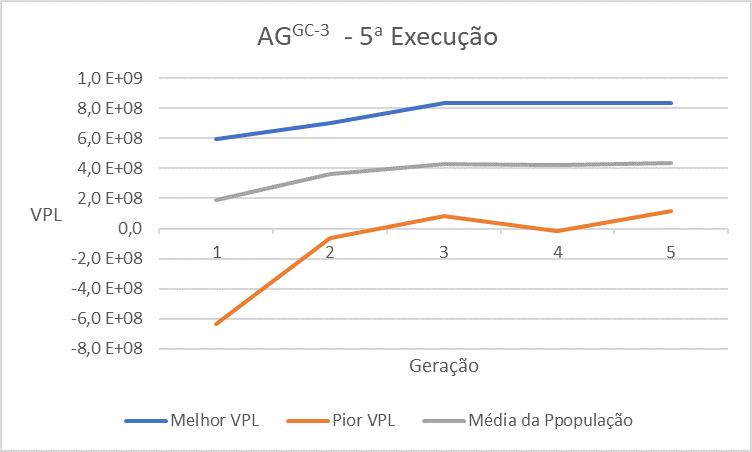
\includegraphics[scale=1]{11}
\caption{Evolução do VPL obtido pela melhor solução, pala pior solução e a média da população obtida na $5^a$ execução do $AG^{GC-3}$}
\label{fig:graph3_2}
\end{figure}

Ao comparar evolução do VPL médio da população e do pior VPL do $AG^{RPC-3}$ (Figura \ref{fig:graph3_1}) e comparar com a evolução da população do $AG^{RPC-2}$ (Figura \ref{fig:graph2_1}), percebe-se que a população do $AG^{RPC-3}$ raramente passa alguma geração sem apresentar uma melhora no fitness médio da população ou no pior fitness, ao contrário do que acontece com o $AG^{RPC-2}$. Quanto à versão geracional do algoritmo, o $AG^{GC-3}$, nota-se que a quantidade de gerações foi consideravelmente reduzida, uma vez que, ao considerar-se uma população com 100 indivíduos, a cada geração, 100 novas avaliações da função objetivo são realizadas, sendo assim são necessários somente 5 gerações dessa versão do AG para atingir o limite de 500 avaliações. Apesar disso, o $AG^{GC-3}$ ainda apresentou um resultado melhor que o das duas versões de AG do experimento anterior. Sendo assim, pode-se afirmar que o aumento da população foi vantajoso para as duas versões do AG, uma vez que esses algoritmos utilizam a população como um repertório para explorar o espaço de busca. Com um repertório maior, a exploração tornou-se mais eficiente.

\subsection{Experimento 4}

A partir dos resultados dos três primeiros experimentos, é possível notar que o AG de Regime Permanente levou ao melhor desempenho até então. Diante disso, essa variação do algoritmo genético foi tomada como base para as alterações da segunda versão do AG apresentada no Capítulo 3.1.2.  Nesse quarto experimento, a tentativa de melhoria dessa versão do algoritmo se deu através da introdução de um novo operador de mutação que utiliza alterações aleatória nos poços da solução com base no IEP de cada poço: a amplitude da alteração realizada em um dado poço é inversamente proporcional ao IEP desse poço, conforme apresentado no Capítulo 3.4. Os demais operadores e parâmetros foram mantidos.

Utilizar o IEP como parâmetro para manipulação dos poços da Estratégia de Produção trouxe grandes melhorias ao desempenho do algoritmo. Como é possível observar nos dados apresentados na Tabela \ref{tab:results1_2} (coluna $AG^{RPM}$), em todas as execuções o VPL obtido foi superior aos resultados obtidos pelos AGs dos experimentos anteriores. A modificação do operador de mutação levou a um ganho de 21,5\% no VPL médio do algoritmo em relação ao experimento anterior. Este ganho observado também foi considerado estatisticamente significativo, segundo o teste de Mann-Whitney-Wilcoxon (considerando um limiar de 5\%), comparando o algoritmo desse experimento com os AGs do experimento anterior. A Tabela \ref{tab:mw4_1} apresenta o resultado do teste estatístico.

\begin{table}[H]
\centering
\caption{Resultados do teste de Mann-Whitney-Wilcoxon para comparar os resultados do $AG^{RPM}$, os AGs do Experimento 3, o $CMOST^500$ e a BA}
\label{tab:mw4_1}
\begin{tabular}{|c|c|c|}
\hline
\multicolumn{2}{|c|}{Algoritmos Comparados} & Resultados \\ \hline
$AG^{RPM}$ & $AG^{RPC-3}$ & 0,0011\% \\ \hline
$AG^{RPM}$ & $AG^{GC-3}$ & 0,0011\% \\ \hline
$AG^{RPM}$ & $CMOST^500$ & 0,0182\% \\ \hline
$AG^{RPM}$ & BA & 0,0011\% \\ \hline


\end{tabular}
\end{table}

No entanto, apesar das melhorias, o algoritmo genético ainda não foi capaz de superar o resultado obtido pelo $CMOST^{500}$. O VPL médio obtido por essa ferramenta ainda é cerca de 33\% superior ao obtido pelo AG desse experimento. Ainda assim, o $AG^{RPM}$ foi capaz de completar as 500 avaliações com um tempo consideravelmente menor, cerca de 38\% do tempo gasto pelo $CMOST^{500}$.

A Figura \ref{fig:graph4_1} apresenta a evolução do VPL da melhor solução, do VPL médio da população e do VPL da pior solução obtidos ao longo da 1a execução dessa versão do algoritmo. É possível notar, pela Figura \ref{fig:graph4_1}, que há evolução do VPL médio da população, basicamente, em todas as iterações, um comportamento semelhante ao observado pelo $AG^{RPC-3}$ no experimento anterior. Vale ressaltar que, para as demais execuções, os gráficos são apresentados no Apêndice D.

\begin{figure}[H]
\centering

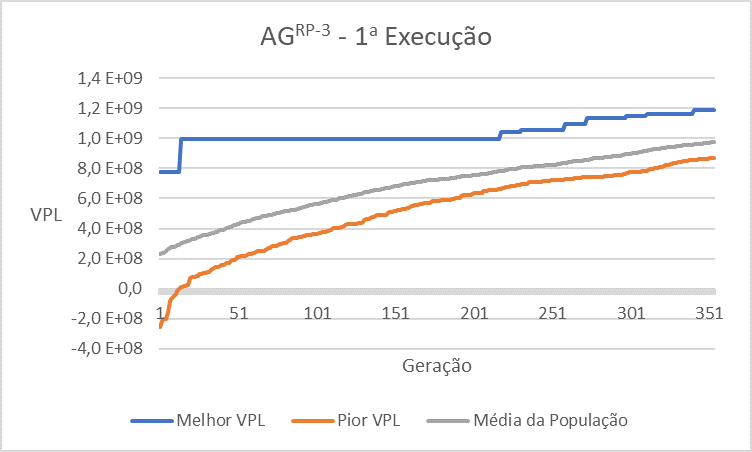
\includegraphics[scale=1]{12}

\caption{Evolução do VPL obtido pela melhor solução, para a pior solução e a média da população obtida na $1^a$ execução do $AG^{RPM}$}
\label{fig:graph4_1}
\end{figure}

\subsection{Experimento 5}

Para o último experimento dessa etapa, foi considerada a terceira versão do algoritmo genético apresentado no Capítulo 3.1.3, que também segue a abordagem de regime permanente. Para testar o conceito proposto para essa versão do AG, foram utilizados dois tamanhos de população: 100 indivíduos ($AG^{CO-1}$) e 50 indivíduos ($AG^{CO-2}$). Tal escolha foi feita, nesse experimento, a fim de se observar como o algoritmo se comporta com o operador proposto no Capítulo 3.6, uma vez que os valores escolhidos para as soluções que compõem a população inicial servem como ponto de partida para esse operador (cálculo do \textit{score}).

O $AG^{CO-2}$ apresentou um VPL médio consideravelmente melhor que o $AG^{CO-1}$ (Tabela \ref{tab:results1_2}). É possível intuir que, com uma população menor a distribuição dos valores para cada intervalo definido para as restrições de posicionamento dos poços foi mais equilibrada. No $AG^{CO-2}$ posições pouco promissoras para os poços podem ter apresentado maior probabilidade de serem escolhidas pelo operador, gerando soluções não tão promissoras. Observando a evolução da população do $AG^{CO-2}$, apresentada na Figura \ref{fig:graph5_2}, percebe-se que a média do VPL da população se aproxima bastante do VPL da melhor solução, mais que o próprio $AG^{CO-1}$, cuja evolução é dada na Figura \ref{fig:graph5_1}, e dos AGs dos experimentos anteriores. Isso pode indicar uma perda da diversidade entre os indivíduos da população, o que não é algo desejado para uma boa exploração do espaço de busca. Apesar do ganho de VPL com a população menor nesse AG, há o risco da perda da diversidade da população. Mais uma vez, os gráficos para as demais execuções das duas versões aqui apresentadas encontram-se no Apêndice E.

\begin{figure}[H]
\centering
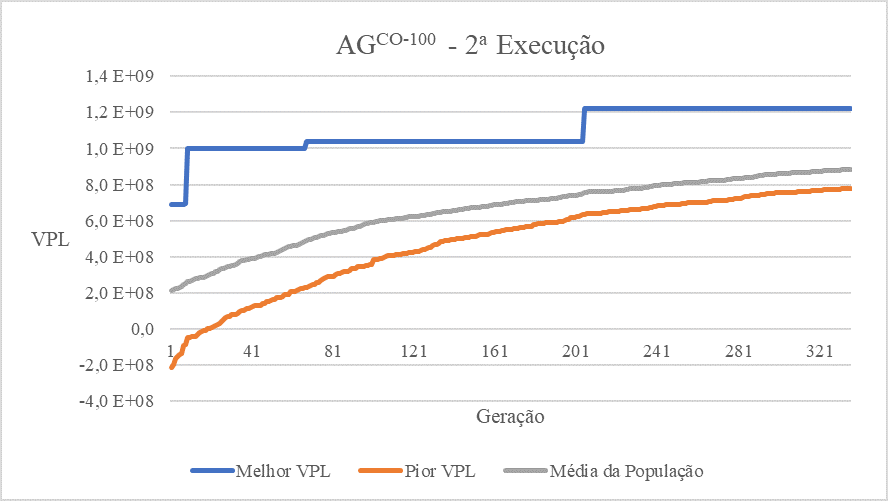
\includegraphics[scale=1]{13}
\caption{Evolução do VPL obtido pela melhor solução, pior solução e a média da população na $2^a$ execução do $AG^{CO-1}$}
\label{fig:graph5_1}
\end{figure}

\begin{figure}[H]
\centering
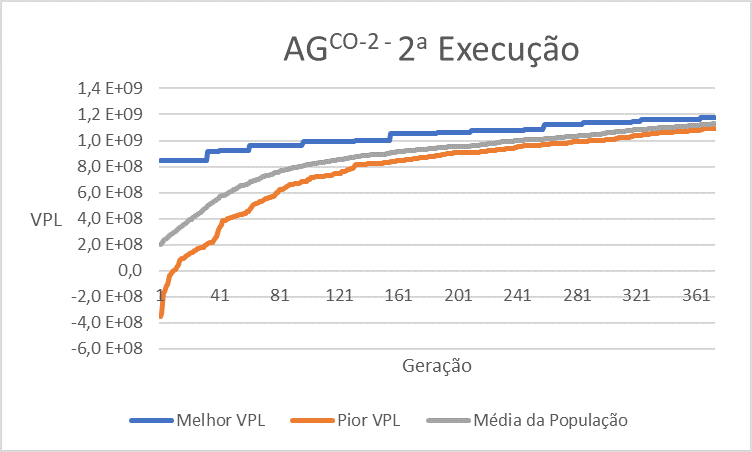
\includegraphics[scale=1]{14}
\caption{Evolução do VPL obtido pela melhor solução, pior solução e a média da população obtida na $2^a$ execução do $AG^{CO-2}$}
\label{fig:graph5_2}
\end{figure}

Ao aplicar o teste de Mann-Whitney-Wilcoxon entre o $AG^{CO-1}$ e o $AG^{CO-2}$, constata-se que a diferença entre os resultados desses AGs é significativa. Mais uma vez utilizando o limiar de 5\%, o teste obteve como resultado 1,40\%.  Tal teste também foi aplicado entre os AGs desse experimento e o $AG^{RPM}$, versão do AG que obteve o melhor resultado até o momento. Os resultados são apresentados na Tabela \ref{tab:mw5_1}.

\begin{table}[H]
\centering
\caption{Resultados do teste de Mann-Whitney-Wilcoxon para comparar os resultados do $AG^{CO-1}$ e do $AG^{CO-2}$ com o $AG^RPM$}
\label{tab:mw5_1}
\begin{tabular}{|c|c|c|}
\hline
\multicolumn{2}{|c|}{Algoritmos Comparados} & Resultados \\ \hline
$AG^{CO-1}$ & $AG^{RPM}$ & 0,10\% \\ \hline
$AG^{CO-2}$ & $AG^{RPM}$ & 6,40\% \\ \hline

\end{tabular}
\end{table}

Como é possível notar pela Tabela \ref{tab:mw5_1}, apesar do $AG^{CO-1}$ ter resultados diferentes e estatisticamente significativos, o $AG^{CO-2}$, que apresentou resultados melhores, não possui uma diferença estatisticamente significativa. Sendo assim, optou-se por não levar adiante essa abordagem.

\section{Etapa 2 – Com Busca Local}

Na segunda etapa dos experimentos o foco esteve na exploração das duas versões da busca local descritas no Capítulo 3.5. No total, foram dois experimentos realizados nessa etapa, sendo que em cada um dos experimentos foi utilizada uma das versões do operador de busca local proposto, em conjunto com o AG que obteve o melhor desempenho na etapa anterior, nesse caso o $AG^{RPM}$ do Experimento 4 da Etapa 1. No primeiro experimento dessa segunda etapa foi utilizado com o $AG^{RPM}$ a primeira versão da busca local ($AG^{BL-1}$). No segundo experimento realizado o AGRPM foi executado com a segunda versão da busca local ($AG^{BL-2}$). Vale ressaltar que os operadores de busca local refinam somente a melhor solução encontrada pelo AG, conforme descrito no Capítulo 3.5.

Apesar da intenção de se comparar os resultados aqui obtidos com os resultados alcançados por $AG^{RPM}$ e  $CMOST^{500}$ na Etapa 1, tal comparação não seria de todo justa. Os AGs dos experimentos realizados nessa etapa precisaram, em média, de um total de 720 avaliações da função objetivo (simulações) para concluir cada execução, 220 avaliações a mais que as utilizadas durante a etapa anterior. Sendo assim, o $AG^{RPM}$ foi executado novamente, mas com um limite de 730 avaliações como critério de parada para que, dessa forma, a comparação fosse justa. O mesmo foi feito para a ferramenta CMOST. Para não haver confusão, o $AG^{RPM}$ executado nessa etapa será referenciado como $AG^{RPM-730}$ e o CMOST como $CMOST^{730}$. 

A Tabela \ref{tab:results2_1} apresenta o melhor VPL obtido por cada uma das dez execuções do $AG^{BL-1}$ e do $AG^{BL-2}$. Além disso, também é apresentado o VPL médio de cada algoritmo, o desvio padrão, o tempo médio, em horas, gasto para cada execução do algoritmo ser concluída e a média de avaliações necessárias para completar a execução dos AGs com busca local. Esses resultados, com exceção da média de avaliações, também são apresentados para $AG^{RPM-730}$ e $CMOST^730$.

\begin{table}[H]
\centering
\caption{Resultados obtidos pela execução dos AGs com Busca Local, do melhor AG da Etapa 1 ($AG^{RPM}$) e do CMOST, ambos com 730 avaliações.}
\label{tab:results2_1}
\begin{tabular}{|c|c|c|c|c|}
\hline
Execução & $AG^{BL-1}$ & $AG^{BL-2}$ & $AG^{RPM-730}$ & $CMOST^730$ \\ \hline
1 & 1,47E+09 & 1,53E+09 & 1,46E+09 & 1,75E+09 \\ \hline
2 & 1,54E+09 & 1,57E+09 & 1,28E+09 & 1,70E+09 \\ \hline
3 & 1,44E+09 & 1,53E+09	& 1,26E+09 & 1,87E+09 \\ \hline
4 & 1,53E+09 & 1,52E+09 & 1,32E+09 & 1,61E+09 \\ \hline
5 & 1,47E+09 & 1,60E+09 & 1,35E+09 & 1,75E+09 \\ \hline
6 & 1,47E+09 & 1,56E+09 & 1,40E+09 & 1,59E+09 \\ \hline
7 & 1,52E+09 & 1,53E+09 & 1,37E+09 & 1,66E+09 \\ \hline
8 & 1,55E+09 & 1,57E+09 & 1,23E+09 & 1,77E+09 \\ \hline
9 & 1,58E+09 & 1,48E+09 & 1,31E+09 & 1,68E+09 \\ \hline
10 & 1,60E+09 & 1,46E+09 & 1,43E+09 & 1,74E+09\\ \hline
Média & 1,52E+09 & 1,53E+09 & 1,34E+09 & 1,71E+09\\ \hline
Desvio Padrão & 5,28E+07 & 4,08E+07 & 7,39E+07 & 8,11E+07\\ \hline
Tempo Médio & 04:18 & 06:17 & 03:49 & 22:50\\ \hline
Média do Avaliações & 720 & 680	 & - & --\\ \hline

\end{tabular}
\end{table}

Os próximos tópicos discutem, com mais detalhes, os experimentos realizados e os resultados obtidos. 


\subsection{Experimento 1}

Como descrito no Capítulo 4.3, nesse experimento o AG foi executado em conjunto com a primeira versão da busca local proposta no Capítulo 3.5. Esse operador de busca local procura, para cada poço da estratégia de produção, verificar uma nova posição em sua vizinhança que leve a ganhos do VPL. Essa busca é realizada até que não haja novas posições que levem a ganhos.

A adição do operador de busca local ao algoritmo genético levou a um ganho de cerca de 29\% do VPL médio quando comparado com o $AG^{RPM}$, executado no Experimento 4 da etapa anterior. O AG com a busca local conseguiu um VPL médio de 1,52E+09 enquanto o $AG^{RPM}$ da Etapa 1 conseguiu um VPL de 1,18E+09. A diferença entre os resultados dessas duas versões do AG é significativa, conforme indica o teste de Mann-Whitney-Wilcoxon, com um limiar de 5\% (Tabela \ref{tab:mw6_1}). No entanto, para que tal resultado fosse obtido, foram necessárias cerca de 220 avaliações a mais e cerca do dobro do tempo utilizado até então.

Em relação ao VPL médio obtido pelo $CMOST^{500}$ na etapa anterior, a diferença fica em torno de 3\%. Sendo que, apesar de ter utilizado um maior número de avaliações, o AG com a busca local precisou, em média, de 4 horas e 18 minutos para concluir uma execução, contra as 7 horas e 15 minutos exigidas pelo $CMOST^{500}$. O AG utiliza cerca de 59\% do tempo gasto pelo $CMOST^{500}$, o que é uma diferença considerável. Os resultados ainda se mostraram estatisticamente significativos conforme o teste de Mann-Whitney-Wilcoxon  (Tabela \ref{tab:mw6_1}).

\begin{table}[H]
\centering
\caption{Resultados do teste de Mann-Whitney-Wilcoxon para comparar os resultados do $AG^{BL-1}$ com o $AG^{RPM}$ e o $CMOST^{500}$.}
\label{tab:mw6_1}
\begin{tabular}{|c|c|c|}
\hline
\multicolumn{2}{|c|}{Algoritmos Comparados} & Resultados \\ \hline
$AG^{BL-1}$ & $AG^{RPM}$ & 2\% \\ \hline
$AG^{BL-1}$ & $CMOST^{500}$ & 1,4\% \\ \hline

\end{tabular}
\end{table}

Apesar dos ganhos apresentados pelo $AG^{BL-1}$, a comparação realizada entre o $AG^{BL-1}$ e o $CMOST^{500}$ não são totalmente justas, uma vez que aqui o $AG^{BL-1}$ realizou cerca de 720 avaliações da função objetivo contra 500 avaliações para os experimentos anteriores. Sendo assim tais algoritmos foram novamente executados com um número maior de avaliações, esse valor passou de 500 para 730. 

Pelos resultados apresentados na Tabela \ref{tab:results2_1} (coluna $AG^{RPM-730}$) é possível afirmar que o operador de busca local utilizado aqui efetivamente leva a um maior VPL, dado que o $AG^{BL-1}$ obteve um VPL Médio cerca de 13\% maior que o obtido pelo $AG^{RPM-730}$. Apesar do $CMOST^{730}$ ter conseguindo um VPL médio cerca de 20\% maior que o $AG^{RPM-730}$ desse experimento e 12,5\% maior que o obtido pelo $AG^{BL-1}$, o $CMOST^{730}$ precisou de cerca de quase 23 horas para concluir todas as 730 avaliações, enquanto que o $AG^{RPM-730}$ utilizou cerca de 17\% desse tempo e o $AG^{BL-1}$ usou somente 19\% desse tempo, uma diferença considerável.

Por fim a diferença entre os resultados obtidos aqui se mostraram significativas ao aplicar o teste de Mann-Whitney-Wilcoxon utilizando um limiar de 5\%. O resultado desse teste é apresentado na Tabela \ref{tab:mw6_2}.

\begin{table}[htb]
\centering
\caption{Resultados do teste de Mann-Whitney-Wilcoxon para comparar os resultados do $AG^{BL-1}$ com o $AG^{RPM-730}$ e o $CMOST^{730}$}
\label{tab:mw6_2}
\begin{tabular}{|c|c|c|}
\hline
\multicolumn{2}{|c|}{Algoritmos Comparados} & Resultados \\ \hline
$AG^{RPM}$  &  $AG^{BL-1}$ & 2\% \\ \hline
$CMOST^{730}$ & $AG^{BL-1}$ & 2,17\% \\ \hline

\end{tabular}
\end{table}

\subsection{Experimento 2}

Para o AG desse experimento, a principal mudança se deu no operador de busca local utilizado. Aqui, a segunda versão desse operador foi escolhida para ser executada com o AG. De uma forma semelhante à primeira versão da busca local, a segunda versão do operador de busca local só termina sua execução caso não exista nenhuma localização, para os poços da estratégia, que melhore a solução. No entanto, o objetivo desse operador é primeiramente melhorar o IEP do poço. O VPL da solução só é considerado caso não seja possível melhorar o IEP do poço alterando sua posição.

O resultado médio obtido pelo $AG^{BL-2}$ não foi muito diferente do obtido pelo $AG^{BL-1}$, já que o VPL obtido foi apenas 1\% melhor. Apesar de ter conseguido concluir com menos avaliações da função objetivo (680 avaliações, em média, contra 720 do $AG^{BL-1}$), o $AG^{BL-2}$ levou mais tempo que o $AG^{BL-1}$, uma diferença de quase 47\%. Ainda assim um tempo consideravelmente menor que o levado pelo $CMOST^{730}$ para concluir as 720 avaliações.

Por fim a diferença entre os resultados do $AG^{BL-2}$ e o $AG^{BL-1}$ não se mostraram estatisticamente significativas segundo o teste de Mann-Whitney-Wilcoxon. Ao aplicar tal teste com a limiar de 5\%, o resultado obtido foi de 52\%.
        
\chapter{Conclusão}
\label{ch:ch6}
De forma geral, o objetivo desse trabalho foi explorar o uso de meta-heurísticas para a resolução do problema de definição de estratégia de produção em campos de petróleo com o intuito de reduzir o esforço computacional para que o algoritmo encontre uma solução de boa qualidade. Para que tal objetivo fosse atingido procurou-se estudar tanto as principais características das meta-heurísticas quanto as principais características do problema em questão para, assim, identificar quais são as informações acerca do problema que podem ser utilizadas para melhorar o processo de otimização realizado pela meta-heurística e como utiliza-los.  

O resultado desse estudo foi apresentado no Capítulo 2 e foi dividido em dois tópicos. O Tópico 2.1 foi dedicado a apresentar os aspectos gerais relacionados as meta-heurísticas, o que difere tais ferramentas de algoritmo clássicos de otimização e quais as situações que o uso de meta-heurísticas é promissor. Além disso, foi apresentado as dificuldades encontradas ao projetar um algoritmo desse tipo, quais as principais meta-heurísticas disponíveis na literatura classificando-as em dois grandes grupos: meta-heurísticas populacionais e de solução única. Por fim, os algoritmos genéticos foram apresentados como a escolha para a resolução do problema, aqui tais algoritmos foram discutidos com mais detalhes, foi apresentado a estrutura básica e os operadores de busca que são necessários para seu funcionamento. Por fim, por se tratar de um algoritmo populacional foi abordado duas estratégias clássicas para a manutenção da população dos algoritmos genéticos: a abordagem geracional, no qual uma nova população é gerada a cada iteração; e a abordagem de regime permanente, onde somente um indivíduo é gerado a cada população e adicionado a população, geralmente, caso seja melhor que algum indivíduo já presente na população. 

Já o Tópico 2 foi destinado a discutir as principais características relativo ao gerenciamento de campos de petróleo, foi abordado aqui as dificuldades para a exploração de campo de petróleo incluindo os riscos e incertezas inerentes a tal atividade. Uma vez apresentado de forma geral o problema, foi apresentado as características operacionais e de infraestrutura necessárias para o sistema de produção para a exploração de um campo de petróleo, em outras palavras, a estratégia de produção adotada para o campo. Além disso, também foi discutido os indicadores técnicos e econômicos utilizados para a avaliação de uma estratégia de produção, que pode ser utilizado para avaliar o sistema como um todo (como o VPL) ou partes do sistema (como os IEPs). Por fim os principais trabalhos realizados para otimização de estratégias de produção utilizando meta-heurísticas foram listados.

Uma vez que foi identificado os principais aspectos das meta-heurísticas, definido os algoritmos genéticos como ponto de partida e levantado as características relacionadas ao problema de DEP, o próximo passo foi realizar modificações ao algoritmo genético e desenvolver novos operadores que utilizam do conhecimento do problema para melhorar o processo de otimização. O resultado dessa etapa foi discutido no Capítulo 3. Aqui foi detalhado as três versões do algoritmo genético utilizadas nesse trabalho: a versão clássica dos AG geracional ($AG^{GC}$) e do AG de Regime Permanente ($AG^(RPC)$) e dois AGs modificados a partir da variação de Regime Permanente, a primeira adaptada para utilizar um novo operador de mutação ($AG^{RPM}$) e a segunda para incluir um novo operador para controlar as ocorrências dos valores definidos para as restrições ($AG^{CO}$). Quanto aos operadores de busca além de operadores clássicos de seleção, recombinação e mutação, foi proposto um novo operador de recombinação e mutação para serem usados com as versões modificadas dos AGs. Além disso, também foi definido aqui a função objetivo e a representação da solução candidata para o problema. Por fim, dois novos operadores foram propostos para auxiliar os AGs no processo de otimização: um operador de busca local e um operador para controlar a ocorrência dos valores das restrições definidas para o problema.

Para que os algoritmos propostos fossem aplicados com sucesso ao problema de DEP foi necessário o uso de algumas ferramentas computacionais como o IMEX, necessário para as simulações de campo de petróleo; o MERO, utilizado para interpretar os resultados da simulações e calcular os indicadores utilizados para a avaliação da soluções candidatas; o jMetal, uma \textit{framewok} que serviu como base para a implementação do AG e seus operadores; e o CMOST, uma ferramenta comercial de otimização que foi utilizado parar ser comparados com os AGs . O Capítulo 4 foi dedicado a detalhar tais ferramentas, além de apresentar o caso de estudo utilizado para validar os algoritmos aqui implementados. Para tal, foi definido em conjunto com o grupo UNISIM, um modelo sintético de reservatório baseado no campo de Namorado, localizado no Rio de Janeiro, os parâmetros econômicos utilizados para a simulação e o escopo do problema para ser resolvido pelos AGs. Tal problema consistiu em encontrar a posição ótima para 18 poços de uma estratégia de produção, sendo dez desses poços do tipo produtor e oito do tipo injetor.

Por fim foi apresentado a estrutura dos experimentos realizados e a configuração dos AGs utilizado em cada experimento. Em resumo, tais experimentos foram divididos em duas etapas: a primeira etapa consiste do uso dos AGs sem o operador de busca local; já para a segunda etapa, tal operador foi considerado em conjunto com o AG que obteve o melhor desempenho durante a primeira etapa. Além disso o número máximo de avaliações foi diferente para cada etapa, para a Etapa 1 foi estabelecido um máximo de 500 avaliações da função objetivo, para a Etapa 2 esse número subiu para um média de 720 avaliações, uma vez que o operador de busca local realiza mais avaliações após a execução do AG. Ao total, foram realizados sete experimentos, sendo cinco durante a primeira etapa e dois durante a segunda etapa. Durante a primeira etapa, os resultados obtidos foram então comparados com uma Busca Aleatória (BA) e com o CMOST executando 500 avaliações da função objetivo ($CMOST^{500}$). Já na segunda etapa, o AG com Busca Local teve seus resultados comparados com o CMOST realizando 730 avaliações ($CMOST^{730}$) e o melhor AG da Etapa 1, também realizando 730 avaliações. Os resultados, então, foram validados através do teste estatístico não-paramétrico de Mann-Whitney-Wilcoxon. 

Enfim, os resultados desses experimentos foram apresentados e discutidos no Capítulo 5. Ao observar os resultados do primeiro experimento da Etapa 1 ficou claro que as versões clássicas tanto do AG Geracional ($AG^{GC-1}$) quanto do AG de Regime Permanente ($AG^{RPC-1}$), junto com os operadores clássicos, não foram capazes de explorar o espaço de busca de forma eficiente.  Ambas as variações do AG não foram capazes de superar o $CMOST^(500)$ e tão pouco a BA. No segundo experimento, ao alterar o operador de recombinação clássico pela proposta apresentada no Tópico 3.5, os AGs clássicos ($AG^{GC-2}$ e $AG^{RPC-2}$) conseguiram um desempenho 17\% melhor que o visto no Experimento 1. No entanto, apesar dos ganhos obtidos pelo novo operador de recombinação, os AGs do Experimento 2 ainda não foram capazes de superar a BA e o $CMOST^(500)$, 

Durante o terceiro experimento, o ajuste de parâmetros levou os AGs ($AG^{GC-3}$ e $AG^{RPC-3}$) a um ganho médio de 24\% em relação AGs do Experimento 2. Com o aumento do tamanho da população os AGs foram capazes de explorar de forma mais eficiente o espaço de busca. Em relação as duas variações utilizadas, o AG de Regime Permanente foi o que mais se beneficiou com tal mudança, garantindo um repertório maior de soluções candidatas melhores, uma vez que só adiciona a população soluções que apresentem alguma melhora em relação a população. A partir desse experimento o AG de Regime Permanente foi definido como base para realizar as modificações ao AG que foi apresentado no Tópico 3.3.2. 

Tal versão modificada do AG ($AG^{RPM}$) foi, então, utilizada durante o Experimento 4. Aqui também foi utilizado o operador de mutação proposto no Tópico 3.6 e que utiliza os Indicadores de Poços como critério para definir a amplitude das modificações aleatória da solução. A estratégia proposta conseguiu um resultado 29\% melhor do que foi obtido no anterior e um desempenho aproximadamente 87\% melhor que a versão clássica dos AG utilizada durante o primeiro experimento, no entanto as mudanças realizadas ainda não foram capazes de superar os resultados obtidos pelo $CMOST$. Para finalizar a primeira etapa de experimentos, foi executado a segunda modificação proposta ao AG apresentada no tópico 3.3.3, a principal alteração dessa versão do AG ($AG^{CO}$) é a inclusão de um operador para contar o número de ocorrências dos valores estabelecidos para as restrições do posicionamento dos poços. Tal informação é utilizada posteriormente ao gerar uma nova solução, a ideia é favorecer os locais mais recorrentes, uma vez que tais locais apresente bons resultados. Os resultados obtidos durante o Experimento 5, no entanto, mostraram que a proposta não foi tão eficaz quanto se esperava. Apesar de ter um desempenho cerca de 76\% melhor que a versão clássica do AG, o $AG^{CO}$, ficou aquém do $AG^{RPM}$, do Experimento 4. Além disso, houve um ganho considerável no tempo gasto para concluir as 500 avaliações em relação aos AGs dos experimentos anteriores.

Apesar dos AGs da Etapa 1 não superarem os resultados obtidos pelo CMOST, executando 500 avaliações da função objetivo, vale ressaltar que o tempo computacional gasto pela ferramenta comercial também foi consideravelmente maior. Enquanto o $AG^{RPM}$, que obteve os melhores resultados entre os AGs, levou cerca de 2 horas e 45 minutos para concluir uma execução, o CMOST precisou de 7 horas e 15 minutos, uma diferença considerável.

Para a segunda etapa dos experimentos somente o $AG^{RPM}$ foi considerado para ser executado com as duas versões do operador de busca local proposto no Tópico 3.7. Vale ressaltar que os parâmetros e os operadores de busca foram os mesmos utilizados pelo AG no experimento da etapa anterior. Como a execução do operador de busca local é uma tarefa computacionalmente cara, optou-se por executá-la somente com a melhor solução encontrada pelo AG. Ainda assim, o número total de avaliações da função objetivo aumentou, em média, para 720 avaliações, sendo 500 o máximo definido para o AG, assim como na etapa anterior, e 220 a quantidade média de avaliações necessárias para a execução da Busca Local.

Para o primeiro experimento da segunda etapa, o AG de Regime Permanente Modificado (proposto no tópico 3.3.2 e utilizado durante o Experimento 4 da Etapa 1) foi executado com a primeira versão da Busca Local. Esse operador procura, para cada poço, uma posição em sua vizinhança que leve a um ganho no VPL da solução, essa busca é feita enquanto houver posições vizinhas que apresentem alguma melhora. Tal estratégia se mostrou efetiva ao observar os resultados obtidos nesse experimento, em relação ao $AG^{RPM}$, o AG de Regime Permanente Modificado com o Operador de Busca Local ($AG^{BL-1}$) conseguiu um resultado médio 29\% melhor. Ao comparar com o resultado do CMOST da Etapa 1, a diferença foi de apenas 3\%. Ainda deve-se considerar que o $AG^{BL-1}$, mesmo realizando mais avaliação que o $CMOST^{500}$, levou cerca de 4 horas e 18 minutos para concluir o processo de otimização, enquanto o $CMOST^(500)$ de cerca de 7 horas para concluir as 500 avaliações da função objetivo.

Apesar dos resultados promissores obtidos pelo $AG^{BL-1}$, a comparação realizada com os resultados do AG e do CMOST da Etapa 1 não foram ao todo justas, uma vez que esses realizaram 500 avaliações da função objetivo, enquanto o $AG^{BL-1}$ teve um média de 720 avaliações da função objetivo. Tendo isso em mente, o $AG^{RPM}$ e o CMOST foram novamente executados dessa vez realizando um máximo de 730 avaliações da função objetivo. Ainda assim, em relação aos resultados obtidos pelo $AG^{RPM}$ nesse experimento($AG^{RPM-730}$), o uso do Operador de Busca Local se mostrou promissor. O $AG^{BL-1}$ apresentou um desempenho cerca de 13,4\% melhor e apesar do uso da busca local ser computacionalmente cara, a diferença de tempo gasto pelo $AG^{BL-1}$ e o $AG^{RPM-730}$ não foi grande, o $AG^(RMP)$ levou cerca de 3 horas 50 minutos para concluir as 730 avaliações, cerca de 30 minutos a menor do tempo gasto pelo $AG^{BL-1}$.

No entanto, o CMOST realizando as 730 avaliações ($CMOST^{730}$), novamente, conseguiu apresentar resultados melhores que o AG, a diferença entre os resultados obtidos pelo $AG^{BL-1}$ e o CMOST chegou a 12,5\%. Contudo, para que o $CMOST^{730}$ conseguisse tal resultado, foi necessário cerca de 22 horas e 50 minutos para concluir as 730 avaliações estabelecidas como critério de parada. O $AG^{BL-1}$ precisou de 19\% do tempo gasto pelo $CMOST^{730}$ para concluir um número equivalente de avaliações.

Para finalizar essa Etapa, foi realizando um segundo experimento utilizando dessa vez uma versão aprimorada do operador de busca local. Essa versão da busca local ainda procura, para cada poço, encontrar posições no reservatório que levem a melhorias na solução. No entanto, ao invés de procurar melhoria no VPL, o operador utilizado aqui, busca primeiramente melhorar o IEP do poço e, caso não encontre novas posições que levem a um ganho do IEP, procurar então posições que levem a um ganho do VPL. O AG com essa versão da Busca Local ($AG^{BL-2}$) obteve um desempenho semelhante a versão original utilizada no experimento anterior, tendo apenas 0,66\% de melhora em relação ao $AG^{BL-1}$.  Nesse experimento, o $AG^{BL-2}$ conseguiu concluir o processo de otimização com menos avaliações da função objetivo que o $AG^{BL-1}$, foram em média 680 avaliações contra 720 do $AG^{BL-1}$, no entanto a estratégia utilizada para a nova versão do operador de busca mostrou-se computacionalmente cara no quesito tempo, uma vez que o $AG^{BL-2}$ precisou de , em média, 6 hora e 17 minutos para concluir cada execução, foram cerca de 2 horas a mais em relação ao tempo gasto pelo $AG^{BL-1}$.
 	
Os experimentos realizados nesse trabalho mostram como os Algoritmos Genéticos são ferramentas robustas e flexíveis. As versões clássicas, tanto com a abordagem Geracional quanto a de Regime Permanente, se mostraram ineficazes ao resolver o problema de definição de estratégia de produção, no entanto, no decorrer dos experimentos foi possível mostrar que com algumas pequenas alterações é possível melhorar o desempenho do AG. Os resultados mais promissores, no entanto, vieram com a inclusão de operadores de busca mais específicos ao problema em questão. Ao manipular os poços da estratégia com base nos IEPs, com o operador de mutação, ou buscar posições que levem a melhores IEPs e ganhos do VPL da solução mais que dobraram em relação os AGs clássicos.
 	
Apesar das soluções encontradas pelo melhor AG, o $AG^{BL-1}$, não terem superado as soluções encontradas pelo CMOST, vale ressaltar que a fermenta comercial precisou de um tempo muito maior para concluir o processo de otimização. Mesmo o $AG^{BL-1}$ realizando mais avaliações que o $CMOST^{500}$, o AG precisou de 4 horas e 18 minutos, em média, para concluir uma execução com 720 avaliações, cerca de 60\% do tempo gasto do $CMOST^{500}$ para concluir 500 avaliações. Nesse cenário, o $CMOST^(500)$ conseguiu uma solução com VPL somente 3\% melhor que a solução obtida pelo $AG^{BL-1}$. Quanto ao $CMOST^{730}$, apesar de ter conseguido soluções com um VPL 12,5\% melhores que o $AG^{BL-1}$, tal ferramenta precisou de quase 23 horas para concluir as 730 uma execução com 730 avaliações da função o objetivo, uma diferença grande quando comparado ao tempo gasto pelo $AG^{BL-1}$ que precisou de cerca de 19\% desse tempo.

Novamente, apesar dos AG aqui implementados não terem superado a ferramenta Comercial CMOST quando se trata das soluções obtidas os AG mostraram-se promissores para a encontrar soluções de qualidade para o problema de definição de estratégia de produção. É possível que com novos ajustes os AG sejam capazes de resultados semelhantes aos obtidos pela fragmenta comercial.  Para que tal objetivo seja atingido, vale estudar o uso de outros indicadores ao processo de otimização. Nesse trabalho foi considerado somente os indicadores de viés econômico para o desenvolvimento dos operadores de busca do AG, não foi considerado, por exemplo, o uso dos indicadores técnicos brevemente citados no Tópico . Os indicadores técnicos podem beneficiar, principalmente, a avaliação dos poços das estratégias de produção uma vez que há indicadores específicos para cada tipo de poço como a Produção de Óleo (que indica a quantidade de óleo produzida por um poço) para o poço produtor e Injeção de Água (que indica a quantidade de água que um poço injetou no reservatório). Utilizar tais indicadores permite uma avaliação mais criteriosa para cada tipo de poço, uma vez que cada um tem papeis distintos no sistema de produção. 

Outro aspecto importante que pode ser explorado pelos operadores durante a busca são as informações proveniente do campo de petróleo. Os indicadores, tanto técnicos quanto econômicos, dizem respeito ao desempenho da estratégia e dos poços, tais indicadores são influenciados pelas propriedades do reservatório como porosidade, permeabilidade e pressão, por exemplo. Cada bloco do modelo do reservatório possui um valor para essa e outras propriedades do campo de petróleo. Estudar correlações entre tais propriedades e os indicadores relacionados aos poços, por exemplo, e inserir tal conhecimento ao processo de otimização pode levar a um posicionamento mais inteligente dos poços da estratégia de produção e, por sua vez, a soluções melhores. Por fim, outro aspecto que merece a atenção é verificar como se comporta os algoritmos desse trabalho com outros modelos de reservatório como, por exemplo, o modelo UNISIM-ID \cite{GasparRavagnani2015}, um modelo mais complexo e mais difícil de encontrar uma solução otimizada.

        % O comando a seguir inclui o arquivo levantamento.tex
        % que contém o capítulo de levantamento bibliográfico. 
        % Detalhe: não precisa incluir a extensão .tex
        % \include{levantamento}
        
        % O comando a seguir inclui o arquivo desenvolvimento.tex
        % que contém o capítulo de desenvolvimento. 
        % Detalhe: não precisa incluir a extensão .tex
        % \include{desenvolvimento}
        
        % O comando a seguir inclui o arquivo conclusoes.tex
        % que contém o capítulo de conclusoes. 
        % Detalhe: não precisa incluir a extensão .tex
        % \include{conclusoes}
        
        
        % Os comandos para as referências bibliográficas estão a seguir
        % Estilo de bibliografia. Nesse caso é o estilo alfabético.
        \bibliographystyle{abntex2-alf}
        % As referências bibliográficas estão no arquivo 
        % bibliografia.bib . Nesse caso, coloque o arquivo sem a
        % extensão .bib.
        \bibliography{bibtex}
        
        % Os anexos, se houver, vêm depois das referências:
        \appendix
        \chapter{Gráficos do Experimento 1}

\subsubsection{Algoritmo Genético Geracional Clásico}
As Figuras \ref{fig:graphGC1-01}-\ref{fig:graphGC1-10} apresentam a evolução do VPL da melhor solução, da pior solução e a média da população das dez execuções do Algoritmo Genético Geracional Clássico durante o Experimento 1 duarnte a Etapa 1 ($AG^{CC-1}$).

\begin{figure}[H]
\centering
\label{fig:graphGC1-01}
\includegraphics[scale=1]{apxA/aggc/1}
\end{figure}

\begin{figure}[H]
\centering
\includegraphics[scale=1]{apxA/aggc/2}
\end{figure}

\begin{figure}[H]
\centering
\includegraphics[scale=1]{apxA/aggc/3}
\end{figure}

\begin{figure}[H]
\centering

\includegraphics[scale=1]{apxA/aggc/4}
\end{figure}
\begin{figure}[htb]
\centering
\includegraphics[scale=1]{apxA/aggc/5}
\end{figure}


\begin{figure}[H]
\centering

\includegraphics[scale=1]{apxA/aggc/6}
\end{figure}

\begin{figure}[H]
\centering

\includegraphics[scale=1]{apxA/aggc/7}
\end{figure}

\begin{figure}[H]
\centering

\includegraphics[scale=1]{apxA/aggc/8}
\end{figure}

\begin{figure}[H]
\centering

\includegraphics[scale=1]{apxA/aggc/9}
\end{figure}

\begin{figure}[H]
\centering
\label{fig:graphGC1-10}
\includegraphics[scale=1]{apxA/aggc/10}
\end{figure}

\subsubsection{Algoritmo Genético de Regime Permanente}
As Figuras 1-10 apresentam a evolução do VPL da melhor solução, da pior solução e a média da população das dez execuções do Algoritmo Genético de Regime Permanente Clássico durante o Experimento 1 da Etapa 1 ($AG^{RPC-1}$).

\begin{figure}[H]
\centering

\includegraphics[scale=1]{apxA/agrpc/1}
\end{figure}

\begin{figure}[H]
\centering

\includegraphics[scale=1]{apxA/agrpc/2}
\end{figure}

\begin{figure}[H]
\centering

\includegraphics[scale=1]{apxA/agrpc/3}
\end{figure}

\begin{figure}[H]
\centering

\includegraphics[scale=1]{apxA/agrpc/4}
\end{figure}

\begin{figure}[H]
\centering

\includegraphics[scale=1]{apxA/agrpc/5}
\end{figure}

\begin{figure}[H]
\centering

\includegraphics[scale=1]{apxA/agrpc/6}
\end{figure}

\begin{figure}[H]
\centering

\includegraphics[scale=1]{apxA/agrpc/7}
\end{figure}

\begin{figure}[H]
\centering

\includegraphics[scale=1]{apxA/agrpc/8}
\end{figure}

\begin{figure}[H]
\centering

\includegraphics[scale=1]{apxA/agrpc/9}
\end{figure}

\begin{figure}[H]
\centering

\includegraphics[scale=1]{apxA/agrpc/10}
\end{figure}
        \chapter{Gráficos do Experimento 2}
As Figuras \ref{fig:graphGC2-01}-\ref{fig:graphGC2-10} apresentam a evolução do VPL da melhor solução, da pior solução e a média da população das dez execuções do Algoritmo Genético Geracional Clássico durante o Experimento 2 da Etapa 1 ($AG^{CC-2}$).

\begin{figure}[H]
\centering
\includegraphics[scale=1]{apxB/aggc/1}
\caption{Primeira execução da versão clássica Algoritmo Genético Geracional com o novo operador de recombinação.}
\label{fig:graphGC2-01}
\end{figure}

\begin{figure}[H]
\centering
\includegraphics[scale=1]{apxB/aggc/2}
\caption{Segunda execução da versão clássica Algoritmo Genético Geracional com o novo operador de recombinação.}
\label{fig:graphGC2-02}
\end{figure}

\begin{figure}[H]
\centering
\includegraphics[scale=1]{apxB/aggc/3}
\caption{Terceira execução da versão clássica Algoritmo Genético Geracional com o novo operador de recombinação.}
\label{fig:graphGC2-03}
\end{figure}

\begin{figure}[H]
\centering
\includegraphics[scale=1]{apxB/aggc/4}
\caption{Quarta execução da versão clássica Algoritmo Genético Geracional com o novo operador de recombinação.}
\label{fig:graphGC2-04}
\end{figure}

\begin{figure}[H]
\centering
\includegraphics[scale=1]{apxB/aggc/5}
\caption{Quinta execução da versão clássica Algoritmo Genético Geracional com o novo operador de recombinação.}
\label{fig:graphGC2-05}
\end{figure}

\begin{figure}[H]
\centering
\includegraphics[scale=1]{apxB/aggc/6}
\caption{Sexta execução da versão clássica Algoritmo Genético Geracional com o novo operador de recombinação.}
\label{fig:graphGC2-06}
\end{figure}

\begin{figure}[H]
\centering
\includegraphics[scale=1]{apxB/aggc/7}
\caption{Sétima execução da versão clássica Algoritmo Genético Geracional com o novo operador de recombinação.}
\label{fig:graphGC2-07}
\end{figure}

\begin{figure}[H]
\centering
\includegraphics[scale=1]{apxB/aggc/8}
\caption{Oitava execução da versão clássica Algoritmo Genético Geracional com o novo operador de recombinação.}
\label{fig:graphGC2-08}
\end{figure}

\begin{figure}[H]
\centering
\includegraphics[scale=1]{apxB/aggc/9}
\caption{Nona execução da versão clássica Algoritmo Genético Geracional com o novo operador de recombinação.}
\label{fig:graphGC2-09}
\end{figure}

\begin{figure}[H]
\centering
\includegraphics[scale=1]{apxB/aggc/10}
\caption{Décima execução da versão clássica Algoritmo Genético Geracional com o novo operador de recombinação.}
\label{fig:graphGC2-10}
\end{figure}

As Figuras 1-10 apresentam a evolução do VPL da melhor solução, da pior solução e a média da população das dez execuções do Algoritmo Genético de Regime Permanente Clássico durante o Experimento 2 da Etapa 1 ($AG^{RPC-2}$).

\begin{figure}[H]
\centering
\includegraphics[scale=1]{apxB/agrpc/1}
\caption{Primeira execução da versão clássica Algoritmo de Regime Permanente com o novo operador de recombinação.}
\label{fig:graphRPC2-01}
\end{figure}

\begin{figure}[H]
\centering
\includegraphics[scale=1]{apxB/agrpc/2}
\caption{Segunda execução da versão clássica Algoritmo de Regime Permanente com o novo operador de recombinação.}
\label{fig:graphRPC2-02}
\end{figure}

\begin{figure}[H]
\centering
\includegraphics[scale=1]{apxB/agrpc/3}
\caption{Terceira execução da versão clássica Algoritmo de Regime Permanente com o novo operador de recombinação.}
\label{fig:graphRPC2-03}
\end{figure}

\begin{figure}[H]
\centering
\includegraphics[scale=1]{apxB/agrpc/4}
\caption{Quarta execução da versão clássica Algoritmo de Regime Permanente com o novo operador de recombinação.}
\label{fig:graphRPC2-04}
\end{figure}

\begin{figure}[H]
\centering
\includegraphics[scale=1]{apxB/agrpc/5}
\caption{Quinta execução da versão clássica Algoritmo de Regime Permanente com o novo operador de recombinação.}
\label{fig:graphRPC2-05}
\end{figure}

\begin{figure}[H]
\centering
\includegraphics[scale=1]{apxB/agrpc/6}
\caption{Sexta execução da versão clássica Algoritmo de Regime Permanente com o novo operador de recombinação.}
\label{fig:graphRPC2-06}
\end{figure}

\begin{figure}[H]
\centering
\includegraphics[scale=1]{apxB/agrpc/7}
\caption{Sétima execução da versão clássica Algoritmo de Regime Permanente com o novo operador de recombinação.}
\label{fig:graphRPC2-07}
\end{figure}

\begin{figure}[H]
\centering
\includegraphics[scale=1]{apxB/agrpc/8}
\caption{Oitava execução da versão clássica Algoritmo de Regime Permanente com o novo operador de recombinação.}
\label{fig:graphRPC2-08}
\end{figure}


\begin{figure}[H]
\centering
\includegraphics[scale=1]{apxB/agrpc/9}
\caption{Nona execução da versão clássica Algoritmo de Regime Permanente com o novo operador de recombinação.}
\label{fig:graphRPC2-09}
\end{figure}

\begin{figure}[H]
\centering
\includegraphics[scale=1]{apxB/agrpc/10}
\caption{Décima execução da versão clássica Algoritmo de Regime Permanente com o novo operador de recombinação.}
\label{fig:graphRPC2-10}
\end{figure}
        \chapter{Primeiro Apêndice}
        % O comando a seguir gera um "dummy text". 
        % Elimine-o quando escrever sua dissertação.
        \lipsum[9]
        
        \chapter{Segundo  Apêndice}
        % O comando a seguir gera um "dummy text". 
        % Elimine-o quando escrever sua dissertação.
        \lipsum[10]
        
        \end{document}
        